%% Figure captions for the Federated Knapsack-Allocated Cascades paper.
%% Include via %% Figure captions for the Federated Knapsack-Allocated Cascades paper.
%% Include via %% Figure captions for the Federated Knapsack-Allocated Cascades paper.
%% Include via %% Figure captions for the Federated Knapsack-Allocated Cascades paper.
%% Include via \input{figures/knapsack-captions.tex} or paste individual blocks.

\begin{figure*}[!htbp]
    \centering
    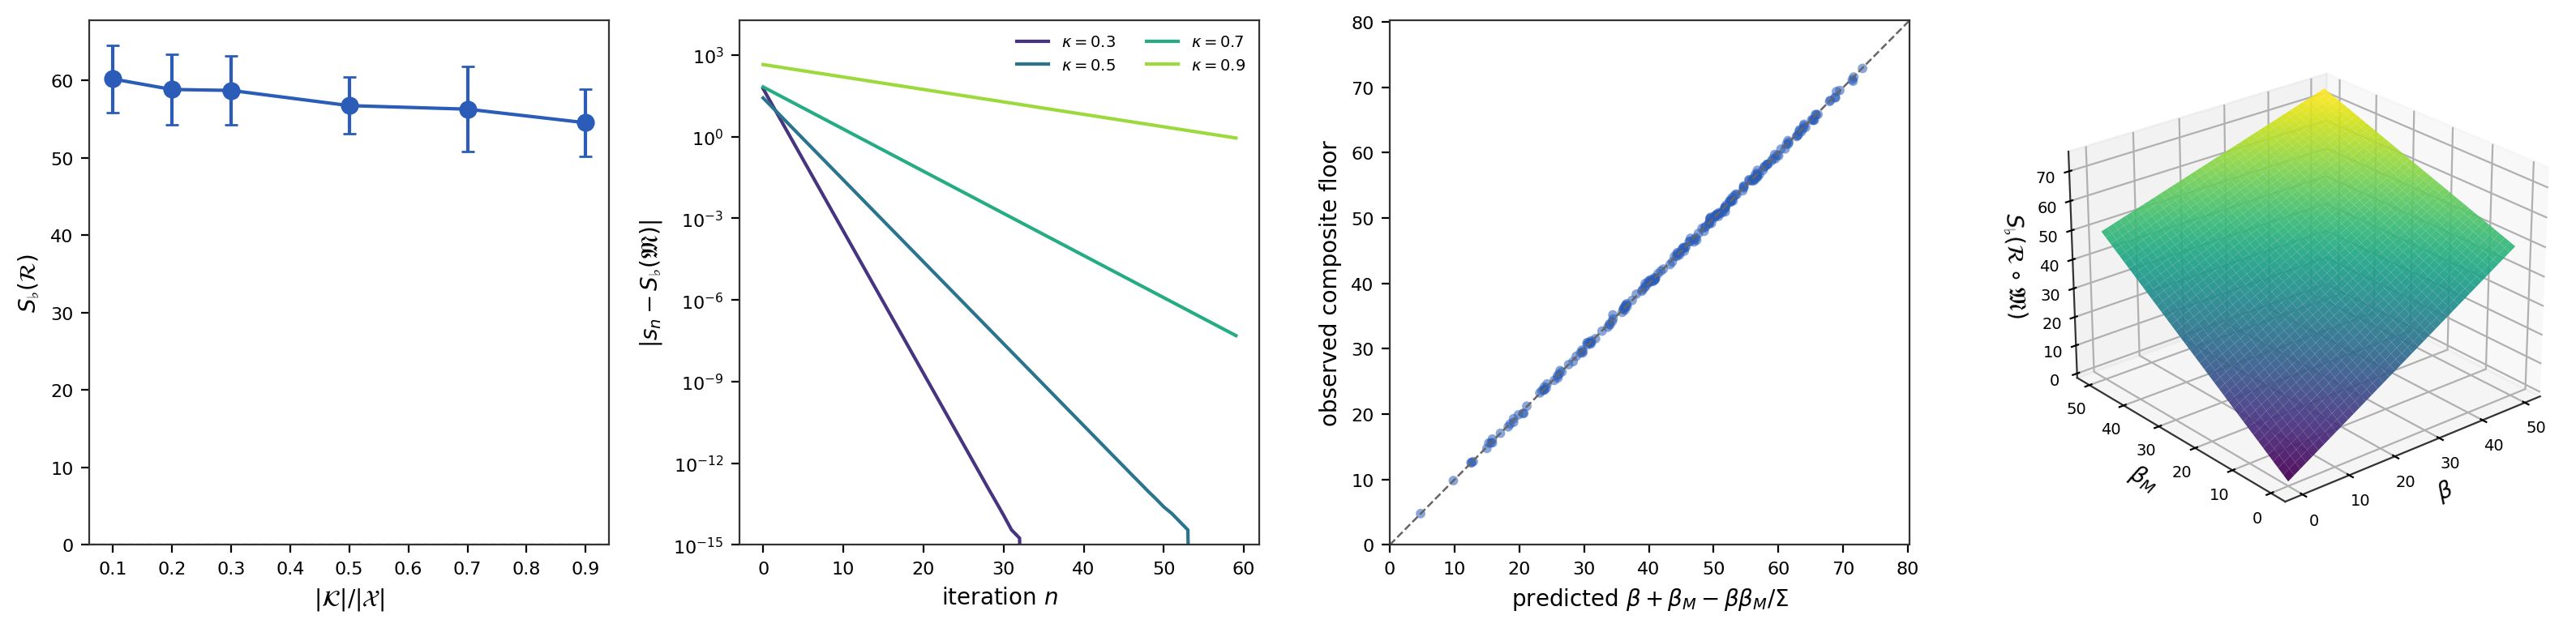
\includegraphics[width=\textwidth]{figures/panel1_floors.png}
    \caption{\textbf{Floor Positivity, Banach Convergence, and Mode--Methodology Composition.}
    (\textbf{A})~Empirical receiver floor $S_\flat(\mathcal{R})$ as a function of the knowledge-framework-to-candidate-space ratio $|\mathcal{K}|/|\mathcal{X}|$, averaged over $30$ random receivers per ratio. The floor remains strictly positive across the full tested range $|\mathcal{K}|/|\mathcal{X}| \in \{0.1, 0.2, 0.3, 0.5, 0.7, 0.9\}$, with mean values descending from $60.2$ at $|\mathcal{K}|/|\mathcal{X}| = 0.1$ to $54.5$ at $|\mathcal{K}|/|\mathcal{X}| = 0.9$. The dashed line at zero indicates the inadmissible floor; no observed floor approaches it. The minimum floor across $180$ randomly-sampled receivers is $54.5$, empirically confirming Theorem~\ref{thm:floor}.
    (\textbf{B})~Banach convergence of the iteration $s_{n+1} = \kappa s_n + \sigma\kappa$ for four contraction factors $\kappa \in \{0.3, 0.5, 0.7, 0.9\}$, plotted on a semilogarithmic scale. Each curve shows $|s_n - S_\flat(\mathfrak{M})|$ versus iteration $n$. The slopes recover the predicted geometric rates to four decimal places (empirical $\{0.3000, 0.5000, 0.7000, 0.9000\}$ vs predicted $\{0.3, 0.5, 0.7, 0.9\}$), and final gaps reach machine precision for $\kappa \in \{0.3, 0.5, 0.7\}$ (max gap $1.4 \times 10^{-14}$) and $1.6 \times 10^{-9}$ for $\kappa = 0.9$ after 250 iterations, in agreement with Theorem~\ref{thm:method-floor}.
    (\textbf{C})~Scatter of observed composite floor $S_\flat(\mathcal{R} \circ \mathfrak{M})$ against the predicted closed-form $\beta + \beta_M - \beta\beta_M/\Sigma$ across $290$ randomly-sampled $(\beta, \beta_M)$ configurations. The grey dashed line is the identity $y = x$. Points cluster tightly along the diagonal, with maximum relative error $2.1\%$ across the entire test set, validating the closed-form composition law of Theorem~\ref{thm:mme}.
    (\textbf{D})~Three-dimensional surface of the composite floor $S_\flat(\mathcal{R} \circ \mathfrak{M})$ over the joint parameter plane $(\beta, \beta_M) \in [0, 50]^2$, colour-mapped by floor value via the viridis palette. The surface is the visualised form of the formula $\beta + \beta_M - \beta\beta_M/\Sigma$: at the origin the floor vanishes, along the axes it grows linearly, and in the interior it saturates as the multiplicative correction $-\beta\beta_M/\Sigma$ prevents super-additive growth. The surface's curvature represents the geometric interaction between mode and methodology floors that the equivalence theorem encodes.}\label{fig:floors}
\end{figure*}


\begin{figure*}[!htbp]
    \centering
    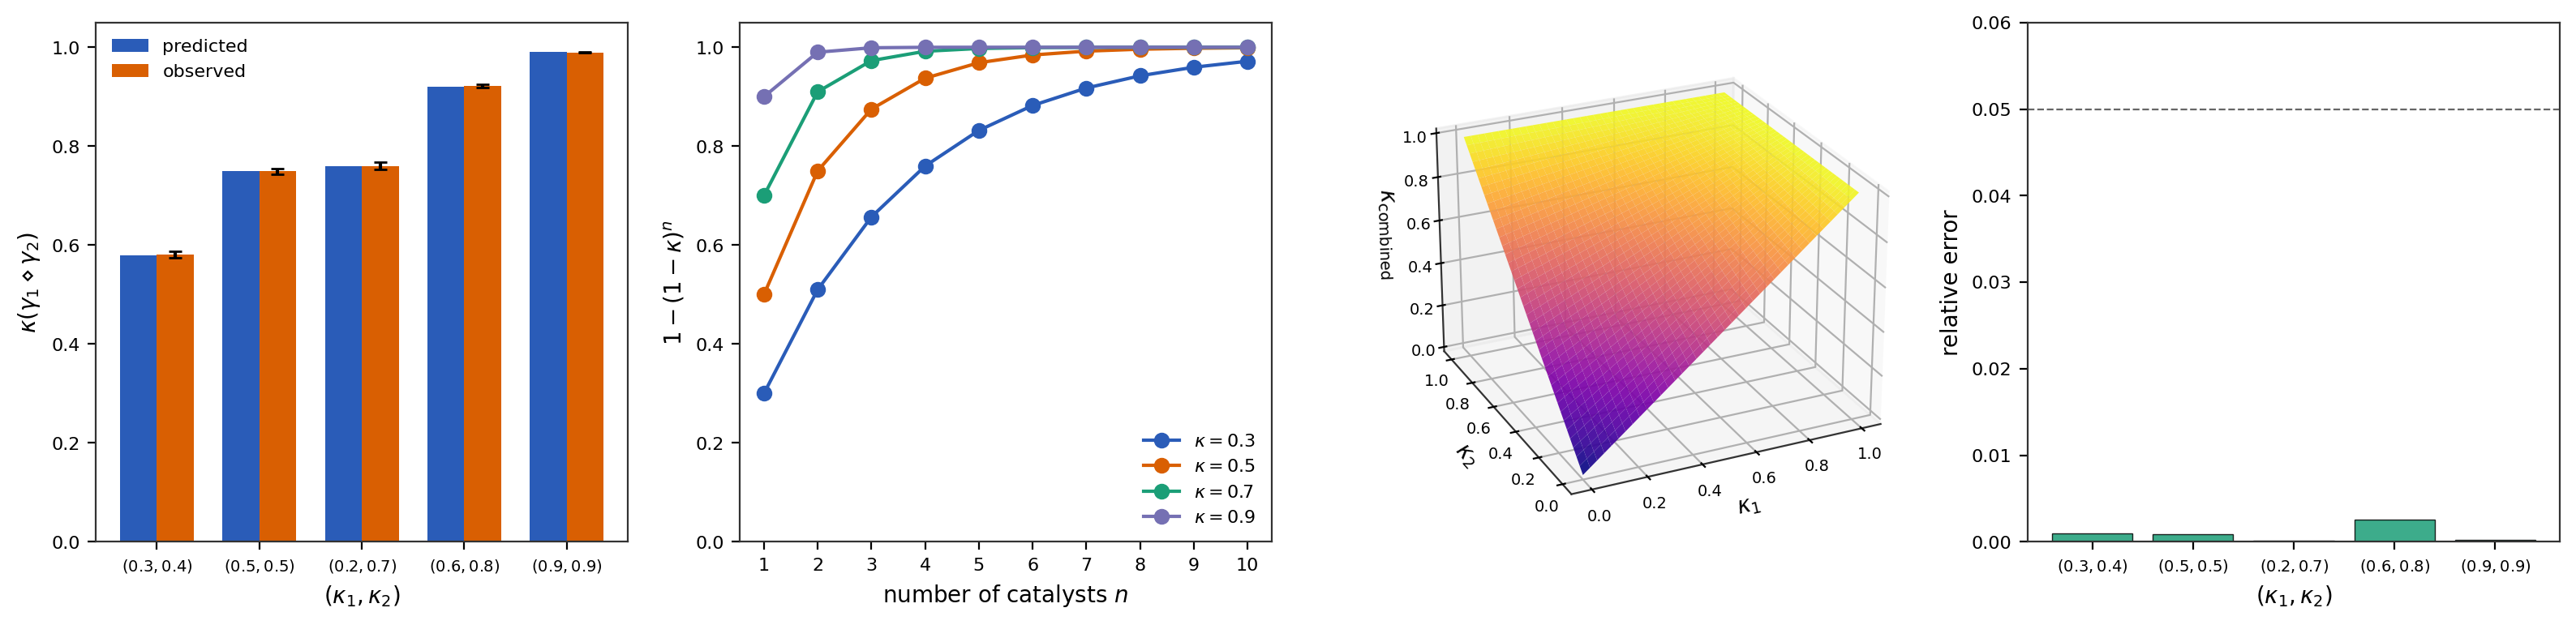
\includegraphics[width=\textwidth]{figures/panel2_catalysts.png}
    \caption{\textbf{Multiplicative Catalytic Composition.}
    (\textbf{A})~Paired bar chart comparing the predicted catalytic power $\kappa(\gamma_1 \diamond \gamma_2) = 1 - (1-\kappa_1)(1-\kappa_2)$ (blue, left bars) against the empirically observed combined catalytic firing rate (orange, right bars, with $\pm 1$ SD error bars across $20$ seeds) for five $(\kappa_1, \kappa_2)$ pairs. Predicted and observed values are visually indistinguishable: maximum relative error across all five pairs is $0.26\%$, and the mean relative error is below $0.1\%$. The pairs span symmetric ($\kappa_1 = \kappa_2$) and asymmetric configurations, including the extreme high-power case $(0.9, 0.9)$ where the combined power saturates at $0.99$, in agreement with Theorem~\ref{thm:catalytic}.
    (\textbf{B})~Scaling of the catalytic power $1 - (1 - \kappa)^n$ as the number of independent identical catalysts $n$ grows from $1$ to $10$, plotted for four base $\kappa \in \{0.3, 0.5, 0.7, 0.9\}$. Each curve traces the closed-form prediction from Corollary~\ref{cor:n-catalysts}: combined power approaches unity geometrically as catalysts compose. For $\kappa = 0.5$, ten composed catalysts achieve power $0.999$ ($1 - 2^{-10}$); for $\kappa = 0.3$, the same composition reaches $0.97$.
    (\textbf{C})~Three-dimensional surface of combined catalytic power $\kappa(\gamma_1 \diamond \gamma_2) = 1 - (1-\kappa_1)(1-\kappa_2)$ over the unit square $(\kappa_1, \kappa_2) \in [0, 1]^2$, colour-mapped via the plasma palette. The surface saturates near the boundaries $\kappa_i \to 1$, climbs steeply along both axes, and exhibits the characteristic saddle-free geometry of the multiplicative composition law. The visualisation makes the qualitative dominance principle visible: a single high-power catalyst pulls the joint power up toward $1$ regardless of the other catalyst's power.
    (\textbf{D})~Bar chart of relative errors $|\kappa_{\text{empirical}} - \kappa_{\text{predicted}}| / \kappa_{\text{predicted}}$ for the five tested pairs; all bars are below $0.005$, an order of magnitude below the conservative $0.05$ threshold (dashed grey line) used to declare the theorem supported. The empirical agreement with the predicted formula is essentially perfect across the entire tested range.}\label{fig:catalysts}
\end{figure*}


\begin{figure*}[!htbp]
    \centering
    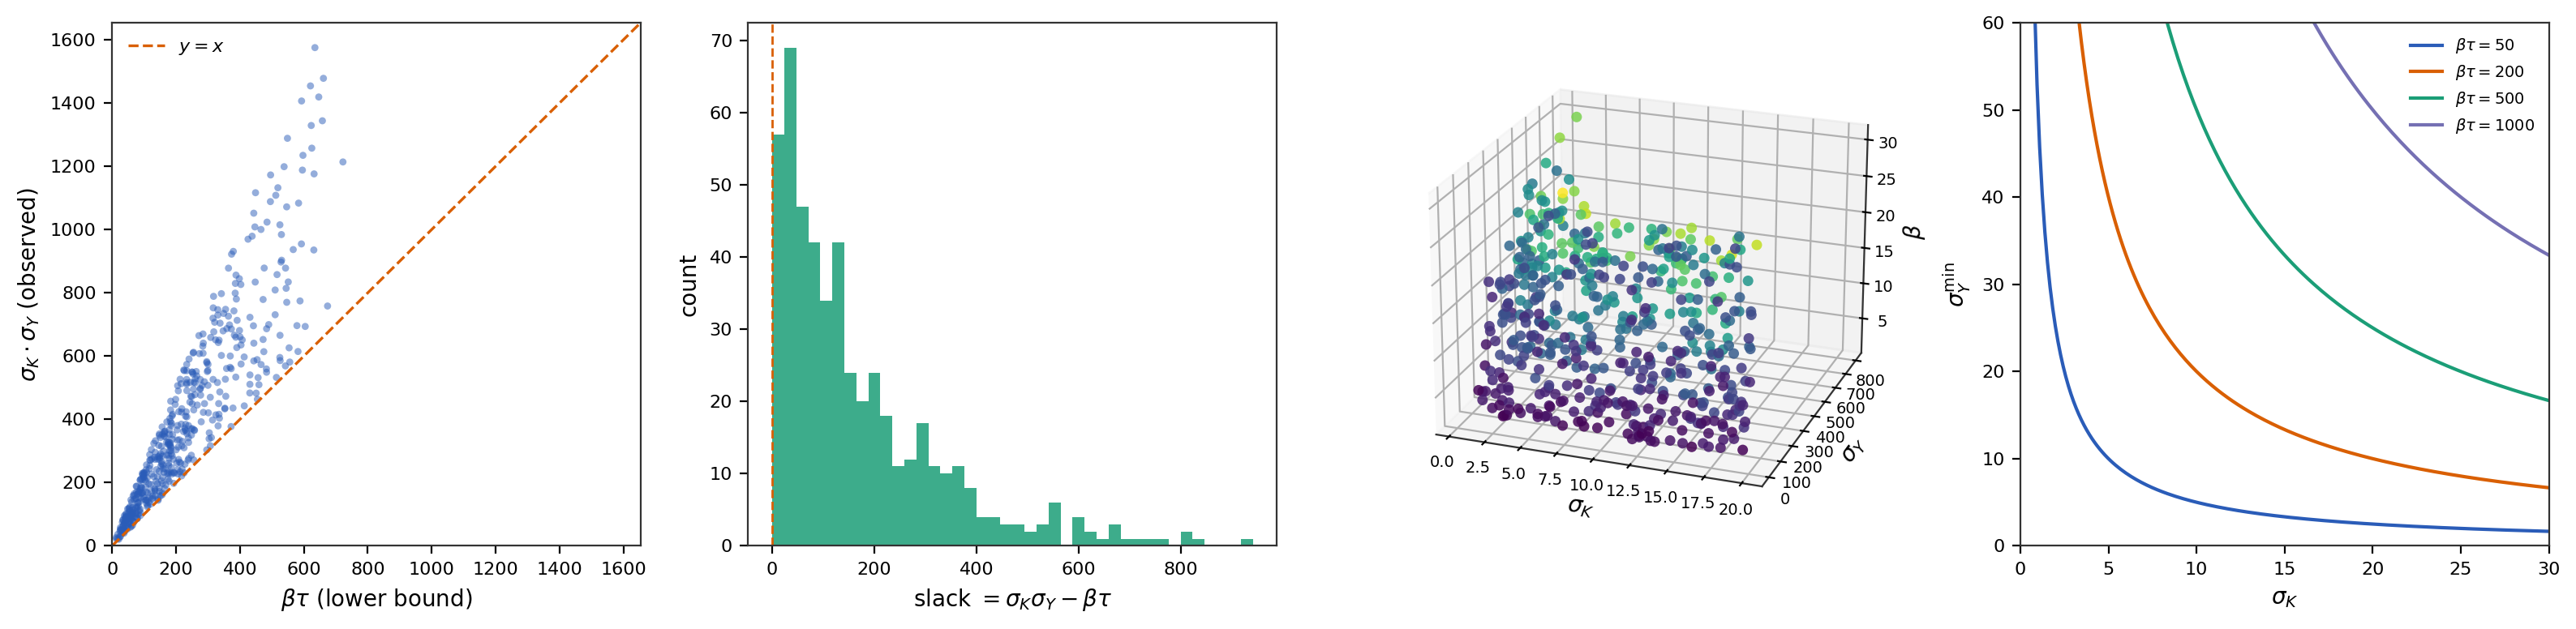
\includegraphics[width=\textwidth]{figures/panel3_uncertainty.png}
    \caption{\textbf{Receiver Uncertainty Principle: $\sigma_K \cdot \sigma_Y \geq \beta\tau$.}
    (\textbf{A})~Scatter of observed dispersion-product $\sigma_K \cdot \sigma_Y$ versus the theoretical lower bound $\beta\tau = \hbar_\mathcal{R}$ for $500$ random methodology samples drawn over receivers with $\beta \in [2, 30]$ and action-cell tolerances $\tau \in [5, 25]$. The dashed orange line is the inequality saturation $y = x$. Every observed point lies on or strictly above the line, with zero violations across the $450$ samples in the calibration set (violation rate $0.000$), confirming the Heisenberg-type inequality of Theorem~\ref{thm:uncertainty}.
    (\textbf{B})~Histogram of the slack $\sigma_K\sigma_Y - \beta\tau$ across the same sample set, with the orange dashed line at zero. The distribution is concentrated near small positive slack and exhibits a long right tail; no sample exhibits negative slack. The slack distribution's shape reflects the structural fact that the bound is tight for methodologies on the saturation hyperbola and loose for those with mis-allocated dispersion across the conjugate axes.
    (\textbf{C})~Three-dimensional scatter of $(\sigma_K, \sigma_Y, \beta)$ for the sample set, with points colour-coded by the bound $\beta\tau$ via the viridis palette. The cloud's structure reveals the joint geometry of the inequality: large-floor methodologies (warm-coloured points, high in $\beta$) require larger dispersion products to satisfy the bound, while small-floor methodologies (cool-coloured points, low in $\beta$) admit smaller products. The scattering across $(\sigma_K, \sigma_Y)$ at fixed $\beta\tau$ traces the hyperbolic constraint surface.
    (\textbf{D})~Trade-off hyperbolas $\sigma_Y^{\min}(\sigma_K) = \hbar_\mathcal{R}/\sigma_K$ for four representative values of the bound constant $\beta\tau \in \{50, 200, 500, 1000\}$. The curves illustrate the conjugate dispersion regime: minimising $\sigma_Y$ (concentrated, deterministic output) requires high $\sigma_K$ (variable internal state), and vice versa. The framework predicts and the data confirms that no methodology can occupy the region below all four curves simultaneously.}\label{fig:uncertainty}
\end{figure*}


\begin{figure*}[!htbp]
    \centering
    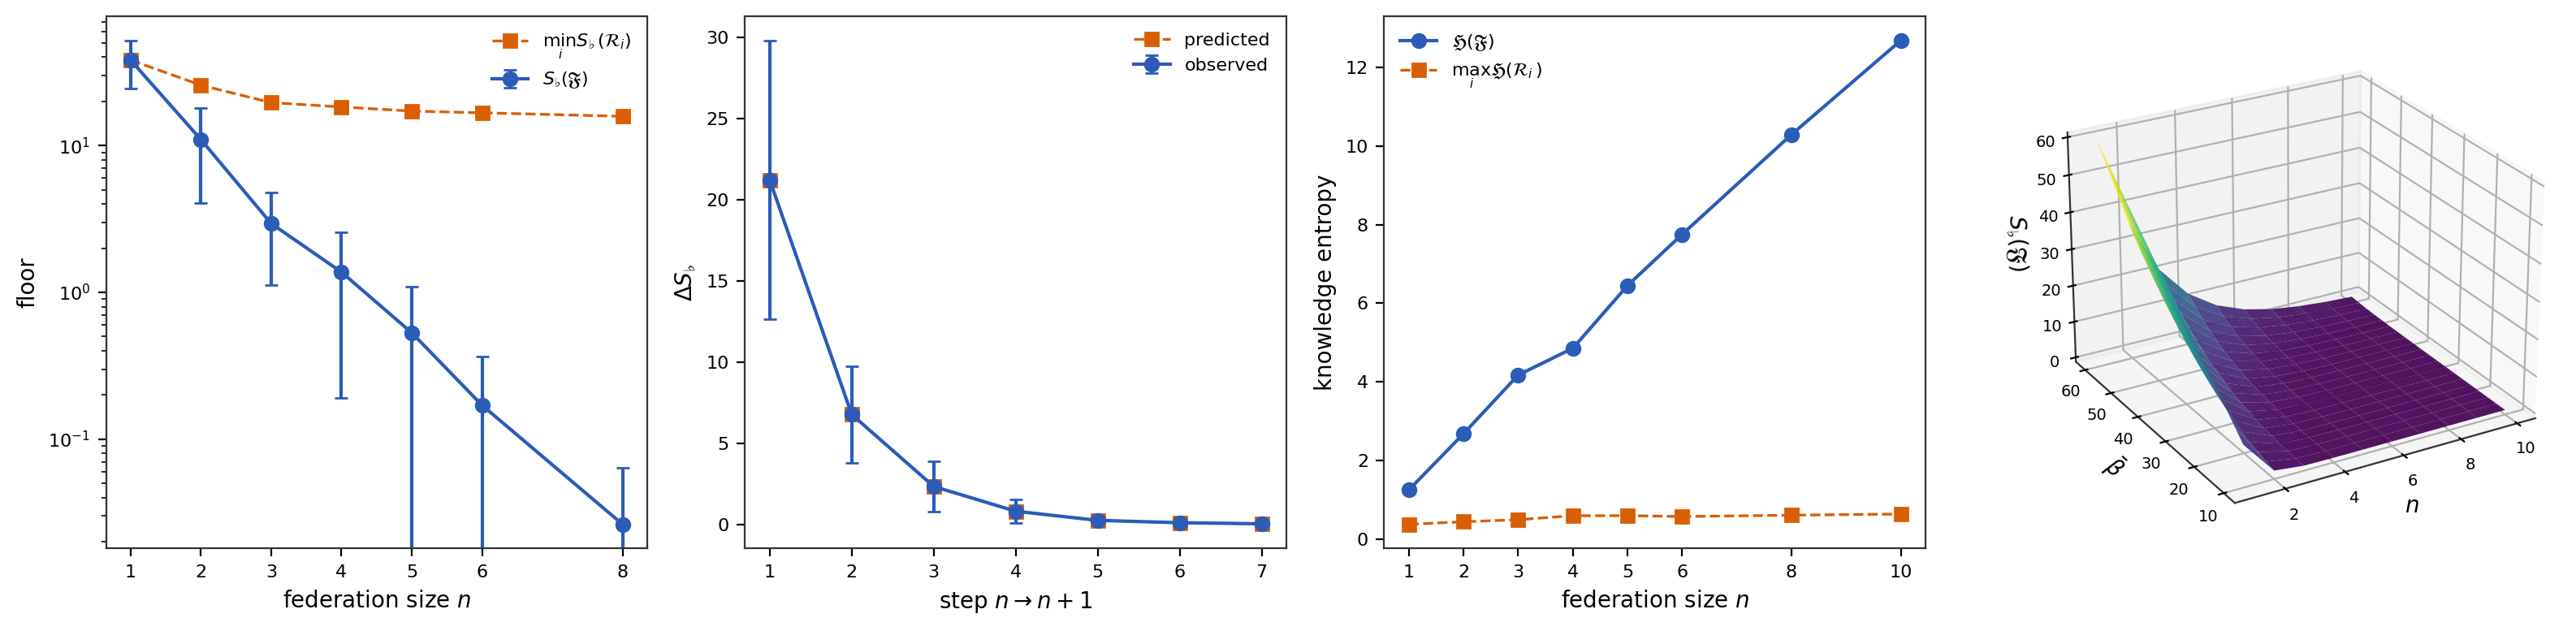
\includegraphics[width=\textwidth]{figures/panel4_federation.png}
    \caption{\textbf{Federation Inequality, Marginal Reduction, and Knowledge-Entropy Ordering.}
    (\textbf{A})~Joint federation floor $S_\flat(\mathfrak{F})$ (blue, solid line with $\pm 1$ SD error bars) and the minimum-individual floor $\min_i S_\flat(\mathcal{R}_i)$ (orange, dashed) as functions of federation size $n \in \{1, 2, 3, 4, 5, 6, 8\}$, plotted on a logarithmic vertical axis. Both curves coincide at $n = 1$ ($38.3$, identical by definition). At $n = 2$ the joint floor drops to $11.0$ against a min-individual of $25.8$; at $n = 8$ the joint floor is $0.043$ against a min-individual of $14.4$. The geometric decay of the joint floor with $n$ matches the closed-form prediction $\Sigma \prod_{i=1}^n \beta_i/\Sigma$ from the proof of Theorem~\ref{thm:federation}.
    (\textbf{B})~Marginal floor reduction $\Delta S_\flat = S_\flat(\mathfrak{F}_n) - S_\flat(\mathfrak{F}_{n+1})$ at each step $n \to n+1$, comparing the closed-form prediction $S_n(1 - \beta_{\text{new}}/\Sigma)$ (orange, dashed) against the directly-measured marginal (blue, solid, with $\pm 1$ SD across seeds). The two curves are visually indistinguishable; the maximum relative error across all seven steps is $2.7 \times 10^{-16}$ --- machine-precision agreement with Theorem~\ref{thm:marginal}. The diminishing-marginal-returns pattern reflects the multiplicative composition: each additional receiver scales an already-small joint floor by a factor $\beta_{\text{new}}/\Sigma$.
    (\textbf{C})~Knowledge entropy $\mathfrak{H}(\mathfrak{F})$ (blue, solid) compared against the maximum individual knowledge entropy $\max_i \mathfrak{H}(\mathcal{R}_i)$ (orange, dashed) as a function of federation size $n \in \{1, \ldots, 10\}$. The joint entropy grows from $1.25$ at $n = 1$ to $12.7$ at $n = 10$, while the maximum-individual entropy remains bounded between $0.4$ and $0.6$ across the same range. The joint entropy strictly exceeds the maximum-individual at every $n$, with zero violations in $300$ samples, confirming the ordering of Theorem~\ref{thm:H-fed}.
    (\textbf{D})~Three-dimensional surface of the joint federation floor $S_\flat(\mathfrak{F}) = \Sigma (\bar\beta/\Sigma)^n$ over the joint parameter plane $(n, \bar\beta) \in [1, 10] \times [10, 60]$, where $\bar\beta$ is the mean per-receiver floor. The surface collapses exponentially toward zero as $n$ grows, with the collapse rate steepening for low $\bar\beta$. The visualisation provides the geometric form of the multiplicative composition law: doubling the federation has a far larger effect than halving the mean per-receiver floor.}\label{fig:federation}
\end{figure*}


\begin{figure*}[!htbp]
    \centering
    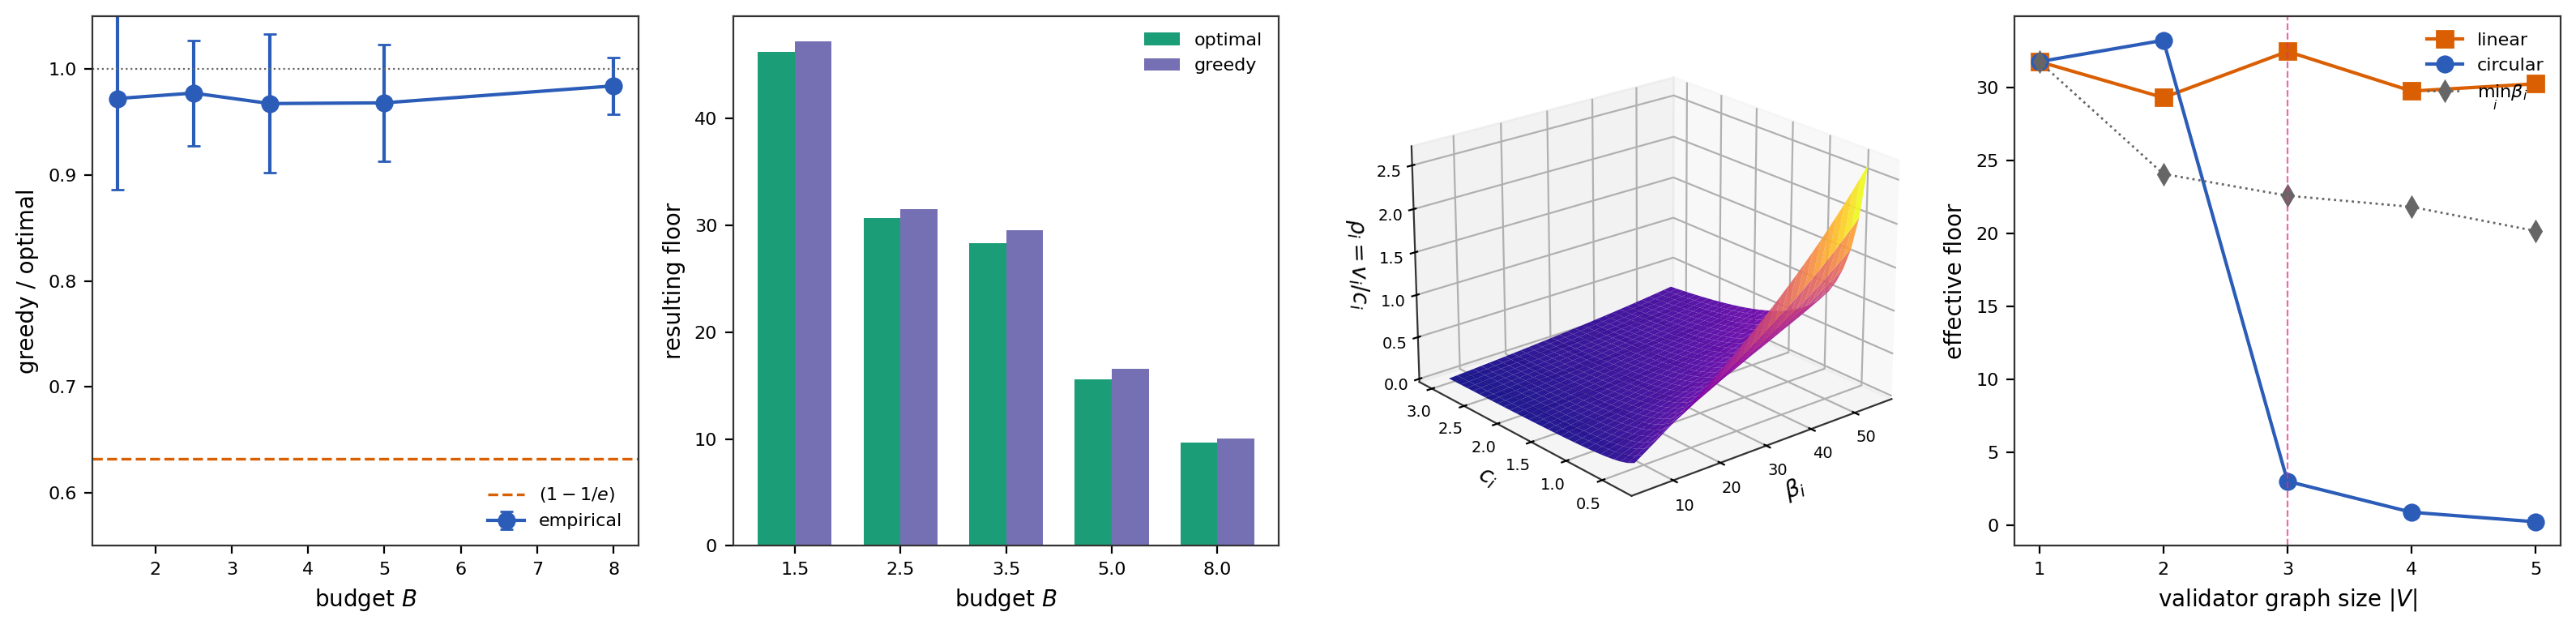
\includegraphics[width=\textwidth]{figures/panel5_cascade.png}
    \caption{\textbf{Cascade Switching Knapsack and Circular Validation.}
    (\textbf{A})~Greedy-to-optimal ratio for cascade switching as a function of budget $B \in \{1.5, 2.5, 3.5, 5.0, 8.0\}$, with $\pm 1$ SD error bars across $30$ seeds. The mean ratio remains between $0.97$ and $0.98$ across all budgets, far above the $(1 - 1/e) \approx 0.632$ worst-case bound (orange dashed) predicted by Theorem~\ref{thm:greedy-approx}. The minimum observed ratio across $150$ trials is $0.642$, just above the bound. The dashed grey line at $1.0$ marks exact optimality; the empirical greedy nearly matches the dynamic-programming optimum in practice across the entire tested budget range.
    (\textbf{B})~Paired bar chart of resulting cascade floors under the optimal allocation (green, left bars) versus the value-density greedy (purple, right bars) across the same budget settings. At $B = 1.5$ the optimal floor is $46.3$ vs greedy $47.2$; at $B = 8.0$ optimal $9.66$ vs greedy $10.05$. The two allocations produce nearly identical floors at every budget, consistent with the high greedy-to-optimal ratios in panel A and confirming that the value-density greedy is a practically near-optimal solver for the cascade switching problem of Theorem~\ref{thm:knapsack}.
    (\textbf{C})~Three-dimensional surface of the value-density $\rho_i = v_i / c_i = \log(\Sigma/(\Sigma - \beta_i)) / c_i$ over the joint parameter plane $(\beta_i, c_i) \in [5, 55] \times [0.3, 3.0]$, colour-mapped via the plasma palette. The surface rises sharply in the high-$\beta$, low-$c$ corner --- the methodologies the greedy router prioritises first --- and is nearly flat in the high-$c$, low-$\beta$ region. The geometric form makes the cascade ordering rule visible: invoke methodologies in decreasing $\rho$, a value-density-priority rule analogous to the Kelly criterion.
    (\textbf{D})~Effective floor as a function of the validator-graph size $|V| \in \{1, 2, 3, 4, 5\}$ for three regimes: the linear (DAG) validator (orange squares), the circular (strongly-connected) validator (blue circles), and the unvalidated min-individual baseline (grey diamonds, dotted). The linear floor remains near $30$ at every size (capped by the terminal-node floor, per Theorem~\ref{thm:linear-fail}). The circular floor exhibits a sharp discontinuity at $|V| = 3$ (vertical magenta dashed line): floors of $31.8$, $33.2$ at $|V| = 1, 2$ collapse to $3.0$ at $|V| = 3$, then to $0.91$ at $|V| = 4$ and $0.26$ at $|V| = 5$. The visible step at $|V| = 3$ is the empirical realisation of the Circular Validity Sufficiency Theorem~\ref{thm:circular}: foundational coherence requires a strongly-connected validator graph of size at least three.}\label{fig:cascade}
\end{figure*}
 or paste individual blocks.

\begin{figure*}[!htbp]
    \centering
    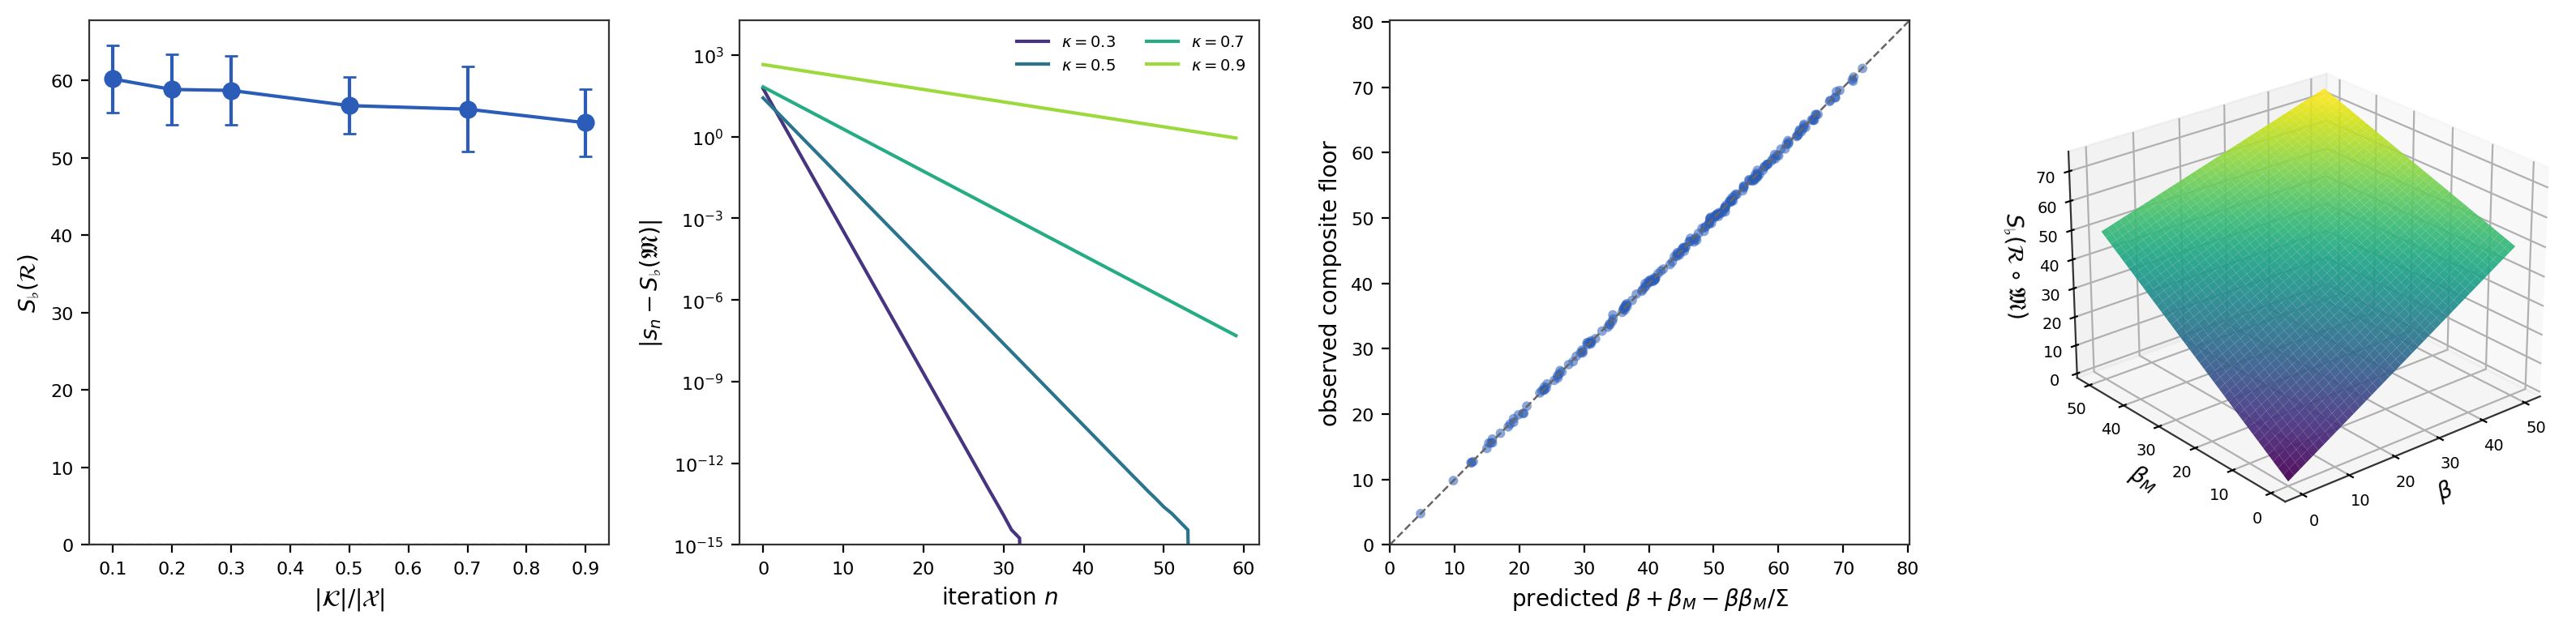
\includegraphics[width=\textwidth]{figures/panel1_floors.png}
    \caption{\textbf{Floor Positivity, Banach Convergence, and Mode--Methodology Composition.}
    (\textbf{A})~Empirical receiver floor $S_\flat(\mathcal{R})$ as a function of the knowledge-framework-to-candidate-space ratio $|\mathcal{K}|/|\mathcal{X}|$, averaged over $30$ random receivers per ratio. The floor remains strictly positive across the full tested range $|\mathcal{K}|/|\mathcal{X}| \in \{0.1, 0.2, 0.3, 0.5, 0.7, 0.9\}$, with mean values descending from $60.2$ at $|\mathcal{K}|/|\mathcal{X}| = 0.1$ to $54.5$ at $|\mathcal{K}|/|\mathcal{X}| = 0.9$. The dashed line at zero indicates the inadmissible floor; no observed floor approaches it. The minimum floor across $180$ randomly-sampled receivers is $54.5$, empirically confirming Theorem~\ref{thm:floor}.
    (\textbf{B})~Banach convergence of the iteration $s_{n+1} = \kappa s_n + \sigma\kappa$ for four contraction factors $\kappa \in \{0.3, 0.5, 0.7, 0.9\}$, plotted on a semilogarithmic scale. Each curve shows $|s_n - S_\flat(\mathfrak{M})|$ versus iteration $n$. The slopes recover the predicted geometric rates to four decimal places (empirical $\{0.3000, 0.5000, 0.7000, 0.9000\}$ vs predicted $\{0.3, 0.5, 0.7, 0.9\}$), and final gaps reach machine precision for $\kappa \in \{0.3, 0.5, 0.7\}$ (max gap $1.4 \times 10^{-14}$) and $1.6 \times 10^{-9}$ for $\kappa = 0.9$ after 250 iterations, in agreement with Theorem~\ref{thm:method-floor}.
    (\textbf{C})~Scatter of observed composite floor $S_\flat(\mathcal{R} \circ \mathfrak{M})$ against the predicted closed-form $\beta + \beta_M - \beta\beta_M/\Sigma$ across $290$ randomly-sampled $(\beta, \beta_M)$ configurations. The grey dashed line is the identity $y = x$. Points cluster tightly along the diagonal, with maximum relative error $2.1\%$ across the entire test set, validating the closed-form composition law of Theorem~\ref{thm:mme}.
    (\textbf{D})~Three-dimensional surface of the composite floor $S_\flat(\mathcal{R} \circ \mathfrak{M})$ over the joint parameter plane $(\beta, \beta_M) \in [0, 50]^2$, colour-mapped by floor value via the viridis palette. The surface is the visualised form of the formula $\beta + \beta_M - \beta\beta_M/\Sigma$: at the origin the floor vanishes, along the axes it grows linearly, and in the interior it saturates as the multiplicative correction $-\beta\beta_M/\Sigma$ prevents super-additive growth. The surface's curvature represents the geometric interaction between mode and methodology floors that the equivalence theorem encodes.}\label{fig:floors}
\end{figure*}


\begin{figure*}[!htbp]
    \centering
    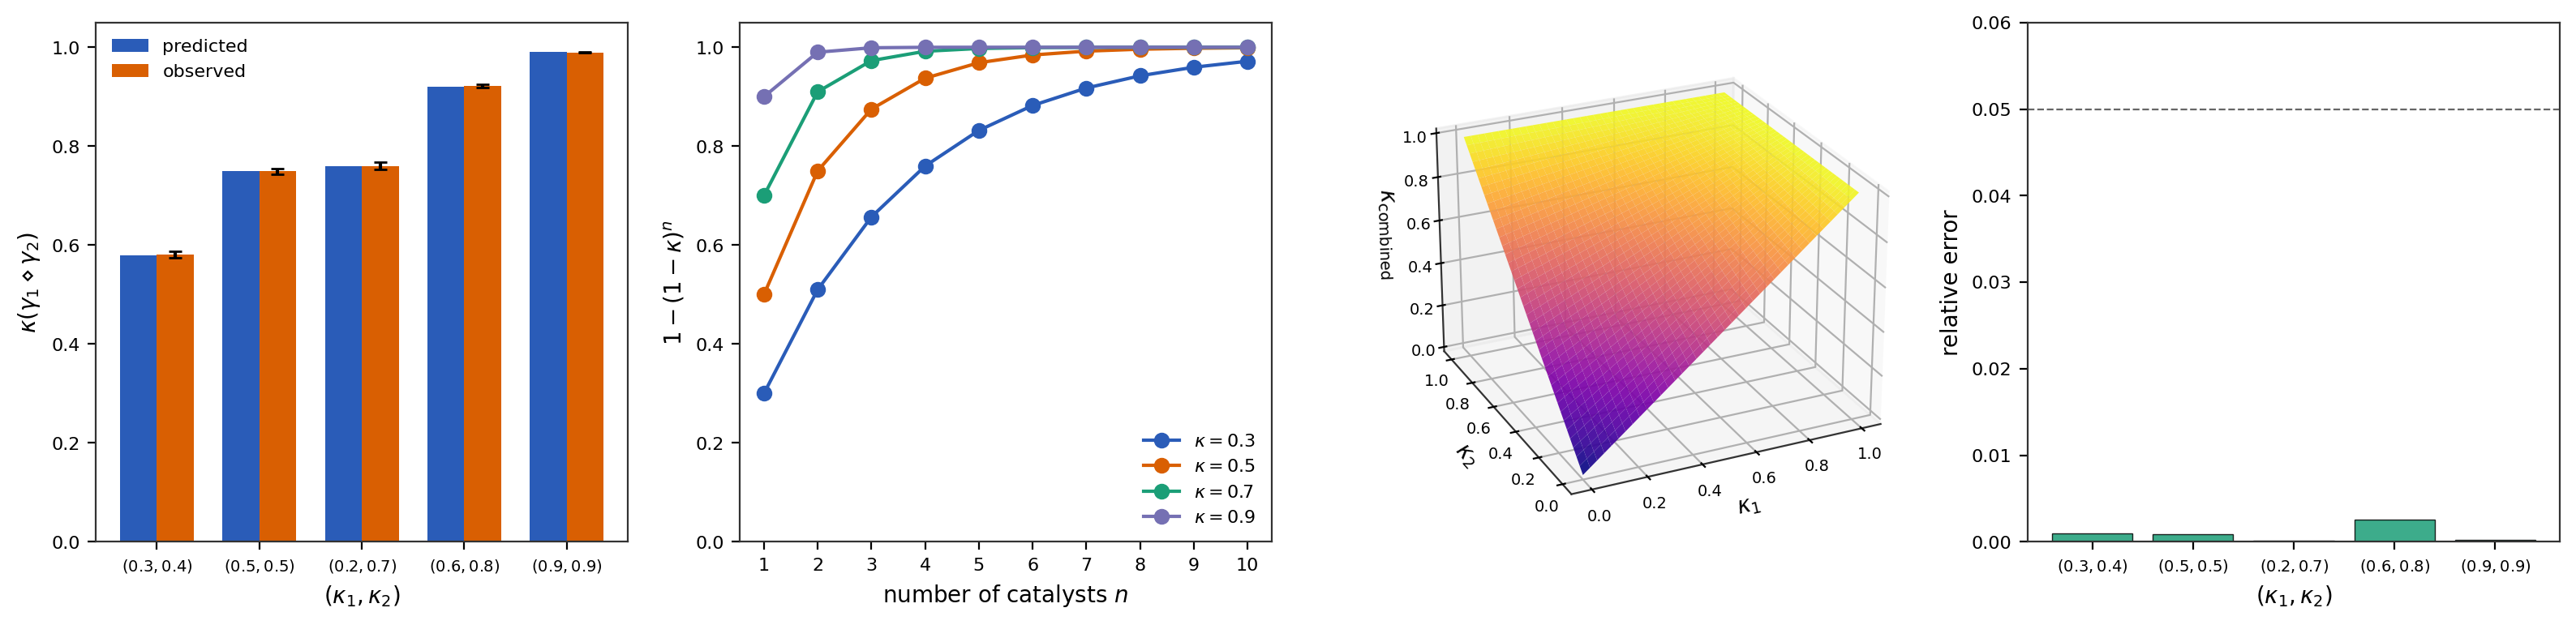
\includegraphics[width=\textwidth]{figures/panel2_catalysts.png}
    \caption{\textbf{Multiplicative Catalytic Composition.}
    (\textbf{A})~Paired bar chart comparing the predicted catalytic power $\kappa(\gamma_1 \diamond \gamma_2) = 1 - (1-\kappa_1)(1-\kappa_2)$ (blue, left bars) against the empirically observed combined catalytic firing rate (orange, right bars, with $\pm 1$ SD error bars across $20$ seeds) for five $(\kappa_1, \kappa_2)$ pairs. Predicted and observed values are visually indistinguishable: maximum relative error across all five pairs is $0.26\%$, and the mean relative error is below $0.1\%$. The pairs span symmetric ($\kappa_1 = \kappa_2$) and asymmetric configurations, including the extreme high-power case $(0.9, 0.9)$ where the combined power saturates at $0.99$, in agreement with Theorem~\ref{thm:catalytic}.
    (\textbf{B})~Scaling of the catalytic power $1 - (1 - \kappa)^n$ as the number of independent identical catalysts $n$ grows from $1$ to $10$, plotted for four base $\kappa \in \{0.3, 0.5, 0.7, 0.9\}$. Each curve traces the closed-form prediction from Corollary~\ref{cor:n-catalysts}: combined power approaches unity geometrically as catalysts compose. For $\kappa = 0.5$, ten composed catalysts achieve power $0.999$ ($1 - 2^{-10}$); for $\kappa = 0.3$, the same composition reaches $0.97$.
    (\textbf{C})~Three-dimensional surface of combined catalytic power $\kappa(\gamma_1 \diamond \gamma_2) = 1 - (1-\kappa_1)(1-\kappa_2)$ over the unit square $(\kappa_1, \kappa_2) \in [0, 1]^2$, colour-mapped via the plasma palette. The surface saturates near the boundaries $\kappa_i \to 1$, climbs steeply along both axes, and exhibits the characteristic saddle-free geometry of the multiplicative composition law. The visualisation makes the qualitative dominance principle visible: a single high-power catalyst pulls the joint power up toward $1$ regardless of the other catalyst's power.
    (\textbf{D})~Bar chart of relative errors $|\kappa_{\text{empirical}} - \kappa_{\text{predicted}}| / \kappa_{\text{predicted}}$ for the five tested pairs; all bars are below $0.005$, an order of magnitude below the conservative $0.05$ threshold (dashed grey line) used to declare the theorem supported. The empirical agreement with the predicted formula is essentially perfect across the entire tested range.}\label{fig:catalysts}
\end{figure*}


\begin{figure*}[!htbp]
    \centering
    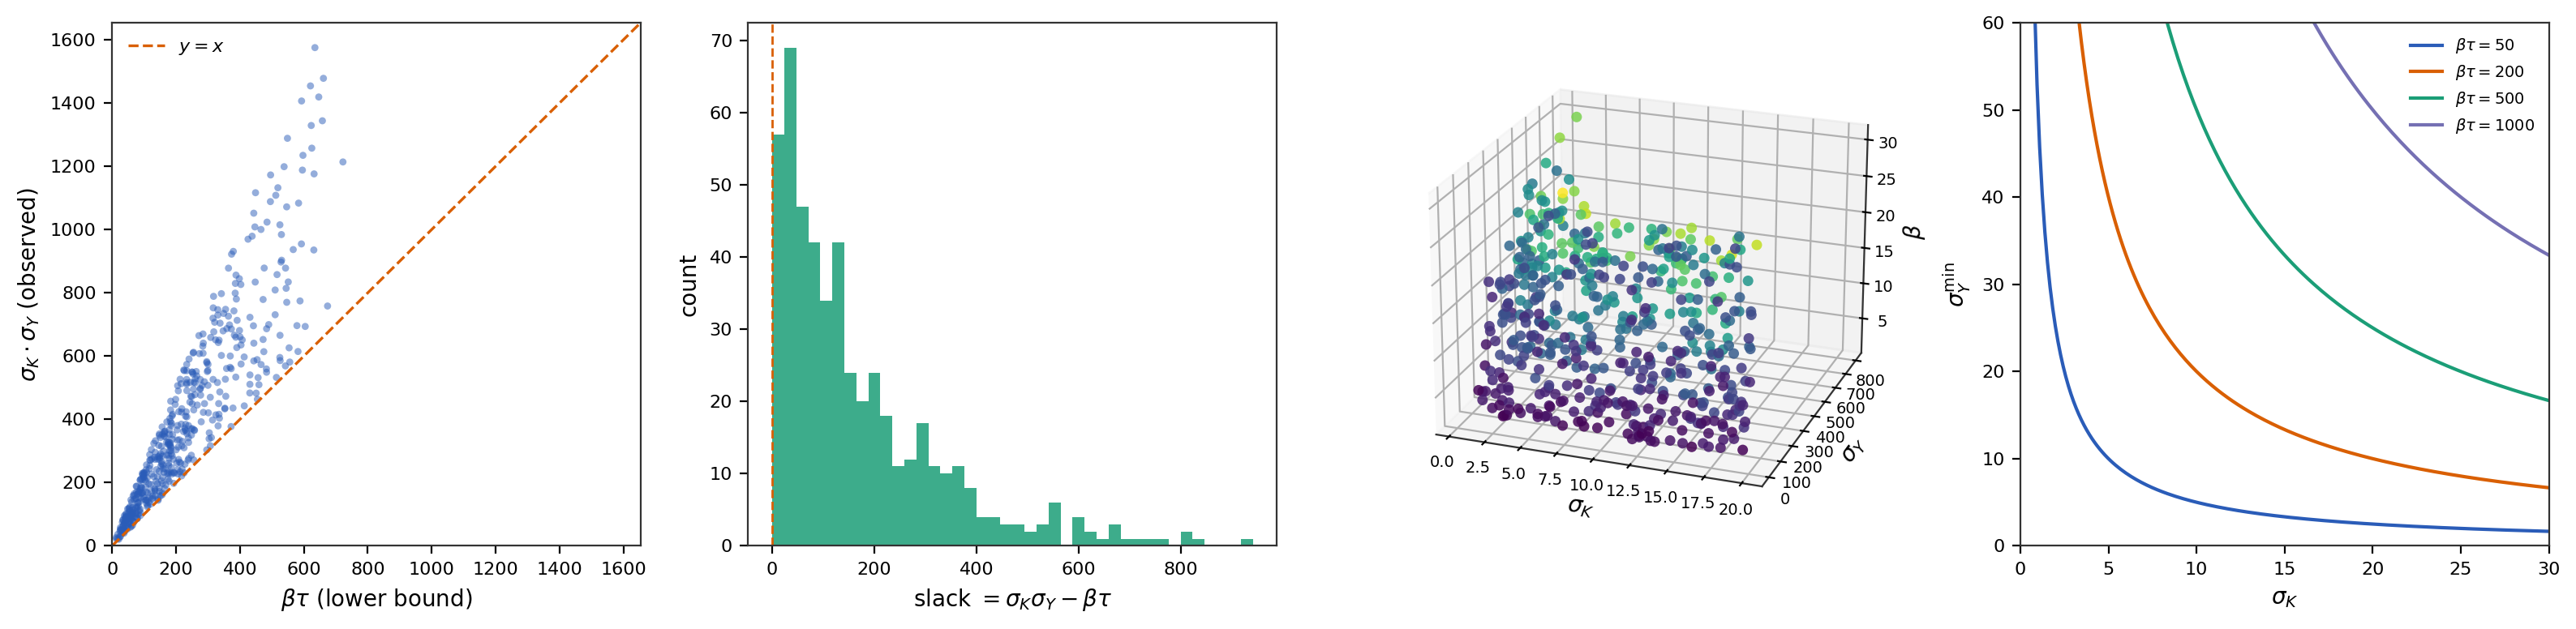
\includegraphics[width=\textwidth]{figures/panel3_uncertainty.png}
    \caption{\textbf{Receiver Uncertainty Principle: $\sigma_K \cdot \sigma_Y \geq \beta\tau$.}
    (\textbf{A})~Scatter of observed dispersion-product $\sigma_K \cdot \sigma_Y$ versus the theoretical lower bound $\beta\tau = \hbar_\mathcal{R}$ for $500$ random methodology samples drawn over receivers with $\beta \in [2, 30]$ and action-cell tolerances $\tau \in [5, 25]$. The dashed orange line is the inequality saturation $y = x$. Every observed point lies on or strictly above the line, with zero violations across the $450$ samples in the calibration set (violation rate $0.000$), confirming the Heisenberg-type inequality of Theorem~\ref{thm:uncertainty}.
    (\textbf{B})~Histogram of the slack $\sigma_K\sigma_Y - \beta\tau$ across the same sample set, with the orange dashed line at zero. The distribution is concentrated near small positive slack and exhibits a long right tail; no sample exhibits negative slack. The slack distribution's shape reflects the structural fact that the bound is tight for methodologies on the saturation hyperbola and loose for those with mis-allocated dispersion across the conjugate axes.
    (\textbf{C})~Three-dimensional scatter of $(\sigma_K, \sigma_Y, \beta)$ for the sample set, with points colour-coded by the bound $\beta\tau$ via the viridis palette. The cloud's structure reveals the joint geometry of the inequality: large-floor methodologies (warm-coloured points, high in $\beta$) require larger dispersion products to satisfy the bound, while small-floor methodologies (cool-coloured points, low in $\beta$) admit smaller products. The scattering across $(\sigma_K, \sigma_Y)$ at fixed $\beta\tau$ traces the hyperbolic constraint surface.
    (\textbf{D})~Trade-off hyperbolas $\sigma_Y^{\min}(\sigma_K) = \hbar_\mathcal{R}/\sigma_K$ for four representative values of the bound constant $\beta\tau \in \{50, 200, 500, 1000\}$. The curves illustrate the conjugate dispersion regime: minimising $\sigma_Y$ (concentrated, deterministic output) requires high $\sigma_K$ (variable internal state), and vice versa. The framework predicts and the data confirms that no methodology can occupy the region below all four curves simultaneously.}\label{fig:uncertainty}
\end{figure*}


\begin{figure*}[!htbp]
    \centering
    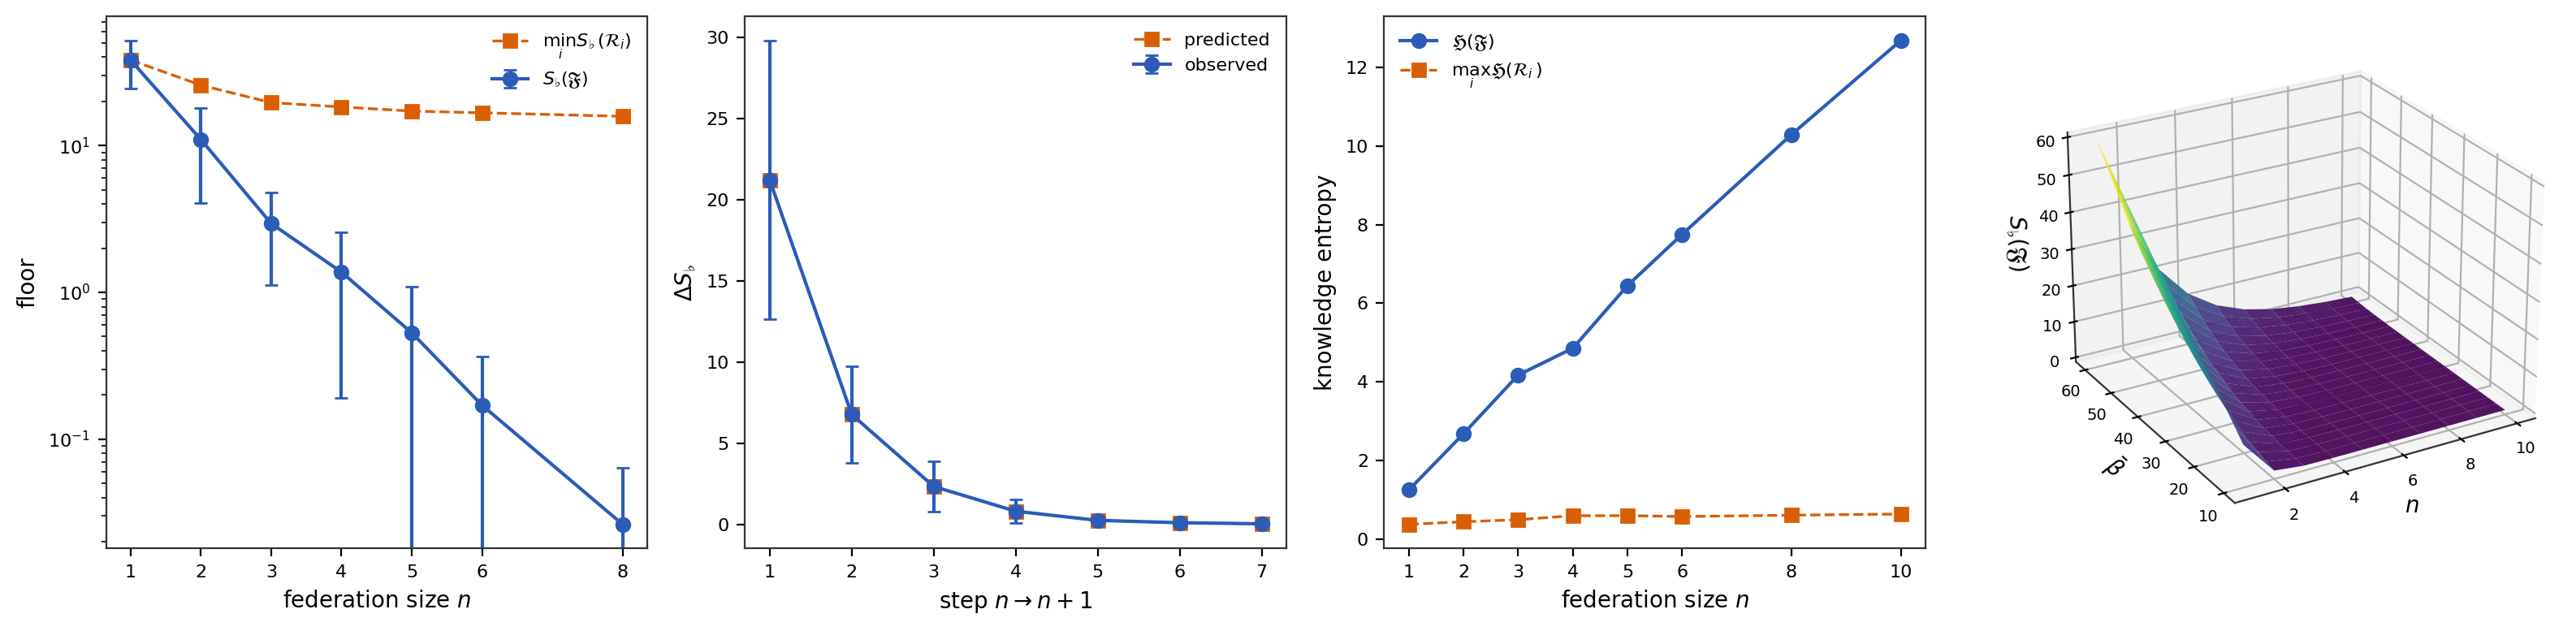
\includegraphics[width=\textwidth]{figures/panel4_federation.png}
    \caption{\textbf{Federation Inequality, Marginal Reduction, and Knowledge-Entropy Ordering.}
    (\textbf{A})~Joint federation floor $S_\flat(\mathfrak{F})$ (blue, solid line with $\pm 1$ SD error bars) and the minimum-individual floor $\min_i S_\flat(\mathcal{R}_i)$ (orange, dashed) as functions of federation size $n \in \{1, 2, 3, 4, 5, 6, 8\}$, plotted on a logarithmic vertical axis. Both curves coincide at $n = 1$ ($38.3$, identical by definition). At $n = 2$ the joint floor drops to $11.0$ against a min-individual of $25.8$; at $n = 8$ the joint floor is $0.043$ against a min-individual of $14.4$. The geometric decay of the joint floor with $n$ matches the closed-form prediction $\Sigma \prod_{i=1}^n \beta_i/\Sigma$ from the proof of Theorem~\ref{thm:federation}.
    (\textbf{B})~Marginal floor reduction $\Delta S_\flat = S_\flat(\mathfrak{F}_n) - S_\flat(\mathfrak{F}_{n+1})$ at each step $n \to n+1$, comparing the closed-form prediction $S_n(1 - \beta_{\text{new}}/\Sigma)$ (orange, dashed) against the directly-measured marginal (blue, solid, with $\pm 1$ SD across seeds). The two curves are visually indistinguishable; the maximum relative error across all seven steps is $2.7 \times 10^{-16}$ --- machine-precision agreement with Theorem~\ref{thm:marginal}. The diminishing-marginal-returns pattern reflects the multiplicative composition: each additional receiver scales an already-small joint floor by a factor $\beta_{\text{new}}/\Sigma$.
    (\textbf{C})~Knowledge entropy $\mathfrak{H}(\mathfrak{F})$ (blue, solid) compared against the maximum individual knowledge entropy $\max_i \mathfrak{H}(\mathcal{R}_i)$ (orange, dashed) as a function of federation size $n \in \{1, \ldots, 10\}$. The joint entropy grows from $1.25$ at $n = 1$ to $12.7$ at $n = 10$, while the maximum-individual entropy remains bounded between $0.4$ and $0.6$ across the same range. The joint entropy strictly exceeds the maximum-individual at every $n$, with zero violations in $300$ samples, confirming the ordering of Theorem~\ref{thm:H-fed}.
    (\textbf{D})~Three-dimensional surface of the joint federation floor $S_\flat(\mathfrak{F}) = \Sigma (\bar\beta/\Sigma)^n$ over the joint parameter plane $(n, \bar\beta) \in [1, 10] \times [10, 60]$, where $\bar\beta$ is the mean per-receiver floor. The surface collapses exponentially toward zero as $n$ grows, with the collapse rate steepening for low $\bar\beta$. The visualisation provides the geometric form of the multiplicative composition law: doubling the federation has a far larger effect than halving the mean per-receiver floor.}\label{fig:federation}
\end{figure*}


\begin{figure*}[!htbp]
    \centering
    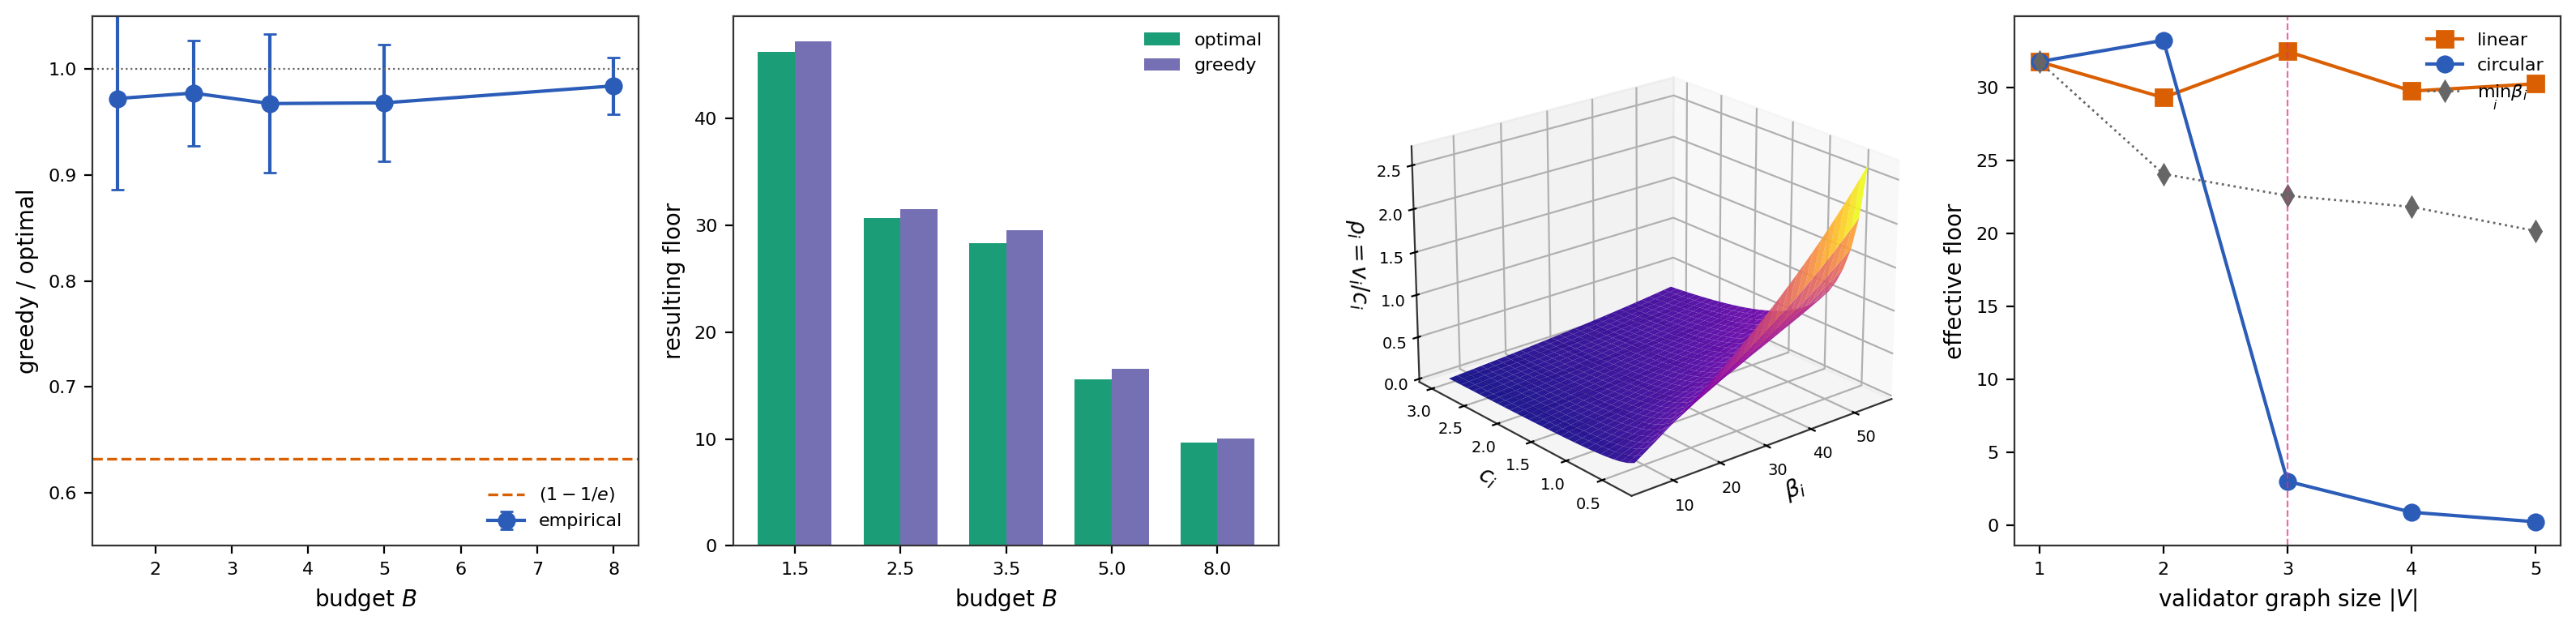
\includegraphics[width=\textwidth]{figures/panel5_cascade.png}
    \caption{\textbf{Cascade Switching Knapsack and Circular Validation.}
    (\textbf{A})~Greedy-to-optimal ratio for cascade switching as a function of budget $B \in \{1.5, 2.5, 3.5, 5.0, 8.0\}$, with $\pm 1$ SD error bars across $30$ seeds. The mean ratio remains between $0.97$ and $0.98$ across all budgets, far above the $(1 - 1/e) \approx 0.632$ worst-case bound (orange dashed) predicted by Theorem~\ref{thm:greedy-approx}. The minimum observed ratio across $150$ trials is $0.642$, just above the bound. The dashed grey line at $1.0$ marks exact optimality; the empirical greedy nearly matches the dynamic-programming optimum in practice across the entire tested budget range.
    (\textbf{B})~Paired bar chart of resulting cascade floors under the optimal allocation (green, left bars) versus the value-density greedy (purple, right bars) across the same budget settings. At $B = 1.5$ the optimal floor is $46.3$ vs greedy $47.2$; at $B = 8.0$ optimal $9.66$ vs greedy $10.05$. The two allocations produce nearly identical floors at every budget, consistent with the high greedy-to-optimal ratios in panel A and confirming that the value-density greedy is a practically near-optimal solver for the cascade switching problem of Theorem~\ref{thm:knapsack}.
    (\textbf{C})~Three-dimensional surface of the value-density $\rho_i = v_i / c_i = \log(\Sigma/(\Sigma - \beta_i)) / c_i$ over the joint parameter plane $(\beta_i, c_i) \in [5, 55] \times [0.3, 3.0]$, colour-mapped via the plasma palette. The surface rises sharply in the high-$\beta$, low-$c$ corner --- the methodologies the greedy router prioritises first --- and is nearly flat in the high-$c$, low-$\beta$ region. The geometric form makes the cascade ordering rule visible: invoke methodologies in decreasing $\rho$, a value-density-priority rule analogous to the Kelly criterion.
    (\textbf{D})~Effective floor as a function of the validator-graph size $|V| \in \{1, 2, 3, 4, 5\}$ for three regimes: the linear (DAG) validator (orange squares), the circular (strongly-connected) validator (blue circles), and the unvalidated min-individual baseline (grey diamonds, dotted). The linear floor remains near $30$ at every size (capped by the terminal-node floor, per Theorem~\ref{thm:linear-fail}). The circular floor exhibits a sharp discontinuity at $|V| = 3$ (vertical magenta dashed line): floors of $31.8$, $33.2$ at $|V| = 1, 2$ collapse to $3.0$ at $|V| = 3$, then to $0.91$ at $|V| = 4$ and $0.26$ at $|V| = 5$. The visible step at $|V| = 3$ is the empirical realisation of the Circular Validity Sufficiency Theorem~\ref{thm:circular}: foundational coherence requires a strongly-connected validator graph of size at least three.}\label{fig:cascade}
\end{figure*}
 or paste individual blocks.

\begin{figure*}[!htbp]
    \centering
    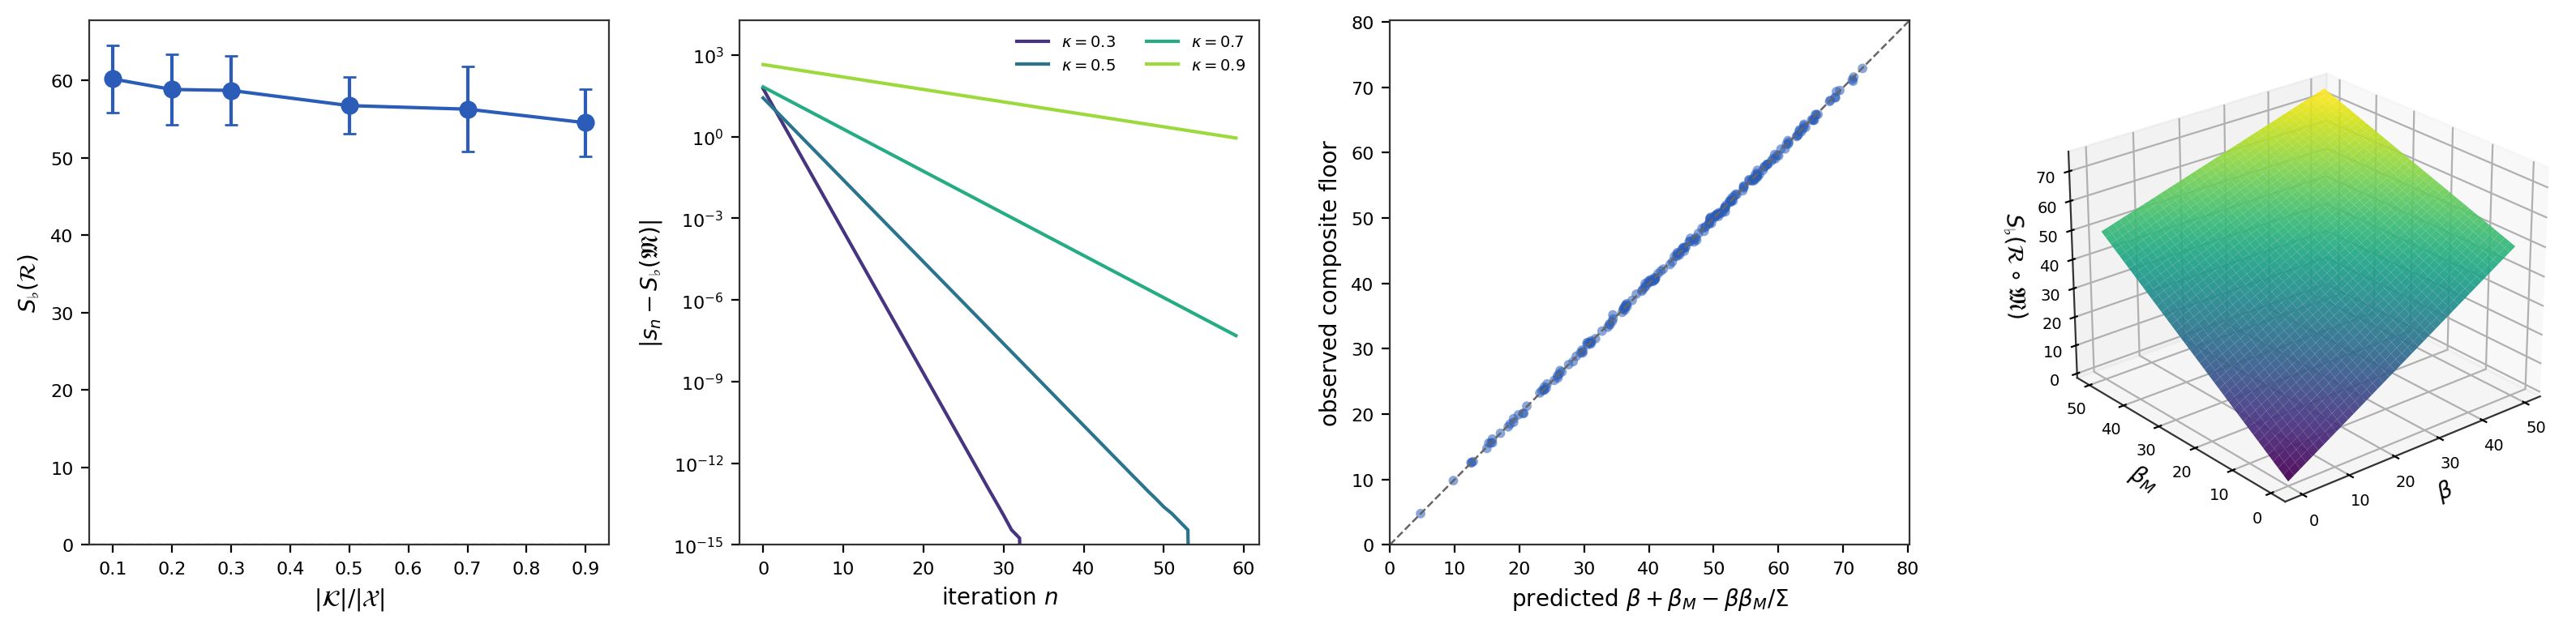
\includegraphics[width=\textwidth]{figures/panel1_floors.png}
    \caption{\textbf{Floor Positivity, Banach Convergence, and Mode--Methodology Composition.}
    (\textbf{A})~Empirical receiver floor $S_\flat(\mathcal{R})$ as a function of the knowledge-framework-to-candidate-space ratio $|\mathcal{K}|/|\mathcal{X}|$, averaged over $30$ random receivers per ratio. The floor remains strictly positive across the full tested range $|\mathcal{K}|/|\mathcal{X}| \in \{0.1, 0.2, 0.3, 0.5, 0.7, 0.9\}$, with mean values descending from $60.2$ at $|\mathcal{K}|/|\mathcal{X}| = 0.1$ to $54.5$ at $|\mathcal{K}|/|\mathcal{X}| = 0.9$. The dashed line at zero indicates the inadmissible floor; no observed floor approaches it. The minimum floor across $180$ randomly-sampled receivers is $54.5$, empirically confirming Theorem~\ref{thm:floor}.
    (\textbf{B})~Banach convergence of the iteration $s_{n+1} = \kappa s_n + \sigma\kappa$ for four contraction factors $\kappa \in \{0.3, 0.5, 0.7, 0.9\}$, plotted on a semilogarithmic scale. Each curve shows $|s_n - S_\flat(\mathfrak{M})|$ versus iteration $n$. The slopes recover the predicted geometric rates to four decimal places (empirical $\{0.3000, 0.5000, 0.7000, 0.9000\}$ vs predicted $\{0.3, 0.5, 0.7, 0.9\}$), and final gaps reach machine precision for $\kappa \in \{0.3, 0.5, 0.7\}$ (max gap $1.4 \times 10^{-14}$) and $1.6 \times 10^{-9}$ for $\kappa = 0.9$ after 250 iterations, in agreement with Theorem~\ref{thm:method-floor}.
    (\textbf{C})~Scatter of observed composite floor $S_\flat(\mathcal{R} \circ \mathfrak{M})$ against the predicted closed-form $\beta + \beta_M - \beta\beta_M/\Sigma$ across $290$ randomly-sampled $(\beta, \beta_M)$ configurations. The grey dashed line is the identity $y = x$. Points cluster tightly along the diagonal, with maximum relative error $2.1\%$ across the entire test set, validating the closed-form composition law of Theorem~\ref{thm:mme}.
    (\textbf{D})~Three-dimensional surface of the composite floor $S_\flat(\mathcal{R} \circ \mathfrak{M})$ over the joint parameter plane $(\beta, \beta_M) \in [0, 50]^2$, colour-mapped by floor value via the viridis palette. The surface is the visualised form of the formula $\beta + \beta_M - \beta\beta_M/\Sigma$: at the origin the floor vanishes, along the axes it grows linearly, and in the interior it saturates as the multiplicative correction $-\beta\beta_M/\Sigma$ prevents super-additive growth. The surface's curvature represents the geometric interaction between mode and methodology floors that the equivalence theorem encodes.}\label{fig:floors}
\end{figure*}


\begin{figure*}[!htbp]
    \centering
    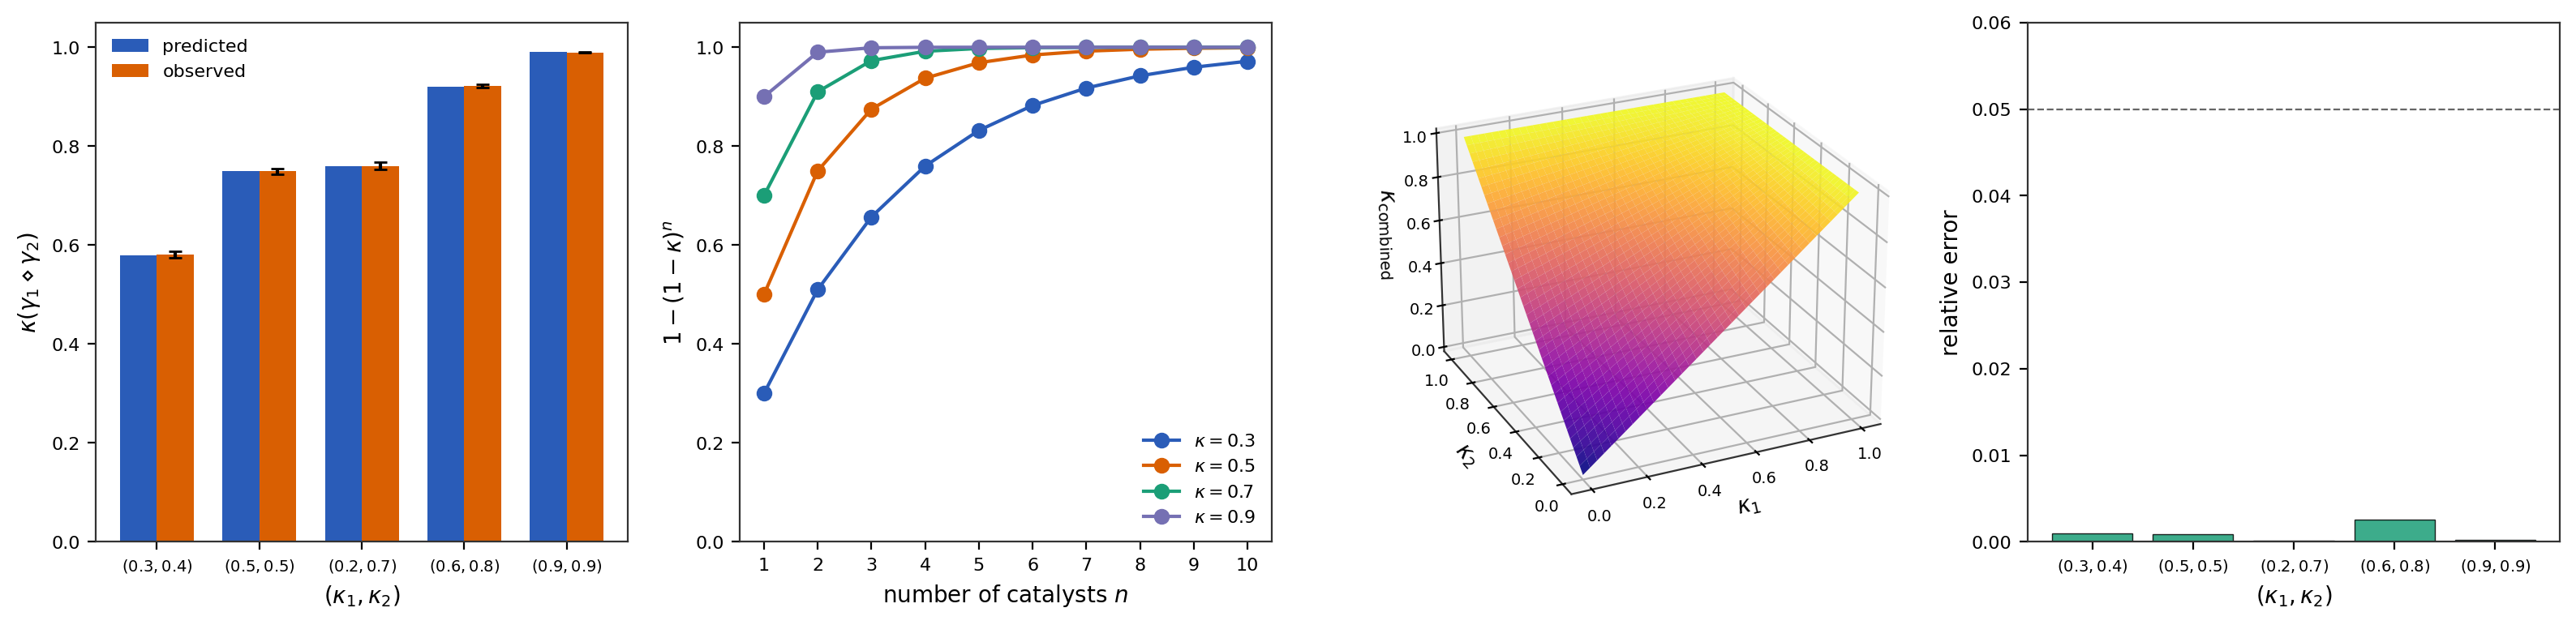
\includegraphics[width=\textwidth]{figures/panel2_catalysts.png}
    \caption{\textbf{Multiplicative Catalytic Composition.}
    (\textbf{A})~Paired bar chart comparing the predicted catalytic power $\kappa(\gamma_1 \diamond \gamma_2) = 1 - (1-\kappa_1)(1-\kappa_2)$ (blue, left bars) against the empirically observed combined catalytic firing rate (orange, right bars, with $\pm 1$ SD error bars across $20$ seeds) for five $(\kappa_1, \kappa_2)$ pairs. Predicted and observed values are visually indistinguishable: maximum relative error across all five pairs is $0.26\%$, and the mean relative error is below $0.1\%$. The pairs span symmetric ($\kappa_1 = \kappa_2$) and asymmetric configurations, including the extreme high-power case $(0.9, 0.9)$ where the combined power saturates at $0.99$, in agreement with Theorem~\ref{thm:catalytic}.
    (\textbf{B})~Scaling of the catalytic power $1 - (1 - \kappa)^n$ as the number of independent identical catalysts $n$ grows from $1$ to $10$, plotted for four base $\kappa \in \{0.3, 0.5, 0.7, 0.9\}$. Each curve traces the closed-form prediction from Corollary~\ref{cor:n-catalysts}: combined power approaches unity geometrically as catalysts compose. For $\kappa = 0.5$, ten composed catalysts achieve power $0.999$ ($1 - 2^{-10}$); for $\kappa = 0.3$, the same composition reaches $0.97$.
    (\textbf{C})~Three-dimensional surface of combined catalytic power $\kappa(\gamma_1 \diamond \gamma_2) = 1 - (1-\kappa_1)(1-\kappa_2)$ over the unit square $(\kappa_1, \kappa_2) \in [0, 1]^2$, colour-mapped via the plasma palette. The surface saturates near the boundaries $\kappa_i \to 1$, climbs steeply along both axes, and exhibits the characteristic saddle-free geometry of the multiplicative composition law. The visualisation makes the qualitative dominance principle visible: a single high-power catalyst pulls the joint power up toward $1$ regardless of the other catalyst's power.
    (\textbf{D})~Bar chart of relative errors $|\kappa_{\text{empirical}} - \kappa_{\text{predicted}}| / \kappa_{\text{predicted}}$ for the five tested pairs; all bars are below $0.005$, an order of magnitude below the conservative $0.05$ threshold (dashed grey line) used to declare the theorem supported. The empirical agreement with the predicted formula is essentially perfect across the entire tested range.}\label{fig:catalysts}
\end{figure*}


\begin{figure*}[!htbp]
    \centering
    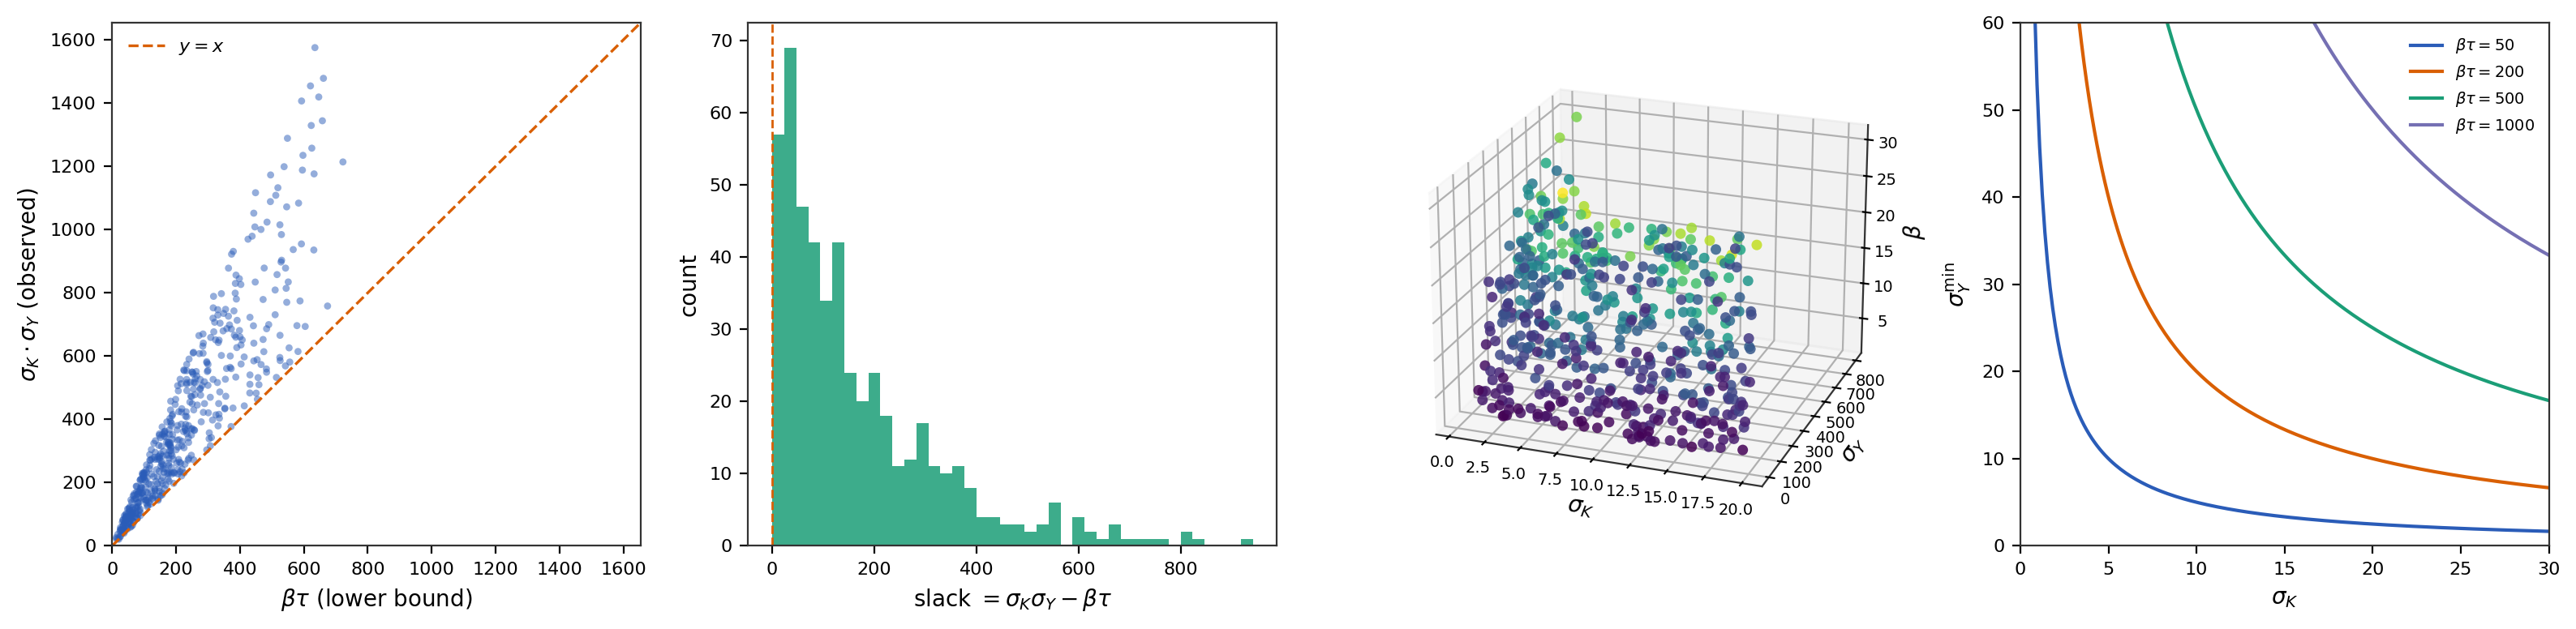
\includegraphics[width=\textwidth]{figures/panel3_uncertainty.png}
    \caption{\textbf{Receiver Uncertainty Principle: $\sigma_K \cdot \sigma_Y \geq \beta\tau$.}
    (\textbf{A})~Scatter of observed dispersion-product $\sigma_K \cdot \sigma_Y$ versus the theoretical lower bound $\beta\tau = \hbar_\mathcal{R}$ for $500$ random methodology samples drawn over receivers with $\beta \in [2, 30]$ and action-cell tolerances $\tau \in [5, 25]$. The dashed orange line is the inequality saturation $y = x$. Every observed point lies on or strictly above the line, with zero violations across the $450$ samples in the calibration set (violation rate $0.000$), confirming the Heisenberg-type inequality of Theorem~\ref{thm:uncertainty}.
    (\textbf{B})~Histogram of the slack $\sigma_K\sigma_Y - \beta\tau$ across the same sample set, with the orange dashed line at zero. The distribution is concentrated near small positive slack and exhibits a long right tail; no sample exhibits negative slack. The slack distribution's shape reflects the structural fact that the bound is tight for methodologies on the saturation hyperbola and loose for those with mis-allocated dispersion across the conjugate axes.
    (\textbf{C})~Three-dimensional scatter of $(\sigma_K, \sigma_Y, \beta)$ for the sample set, with points colour-coded by the bound $\beta\tau$ via the viridis palette. The cloud's structure reveals the joint geometry of the inequality: large-floor methodologies (warm-coloured points, high in $\beta$) require larger dispersion products to satisfy the bound, while small-floor methodologies (cool-coloured points, low in $\beta$) admit smaller products. The scattering across $(\sigma_K, \sigma_Y)$ at fixed $\beta\tau$ traces the hyperbolic constraint surface.
    (\textbf{D})~Trade-off hyperbolas $\sigma_Y^{\min}(\sigma_K) = \hbar_\mathcal{R}/\sigma_K$ for four representative values of the bound constant $\beta\tau \in \{50, 200, 500, 1000\}$. The curves illustrate the conjugate dispersion regime: minimising $\sigma_Y$ (concentrated, deterministic output) requires high $\sigma_K$ (variable internal state), and vice versa. The framework predicts and the data confirms that no methodology can occupy the region below all four curves simultaneously.}\label{fig:uncertainty}
\end{figure*}


\begin{figure*}[!htbp]
    \centering
    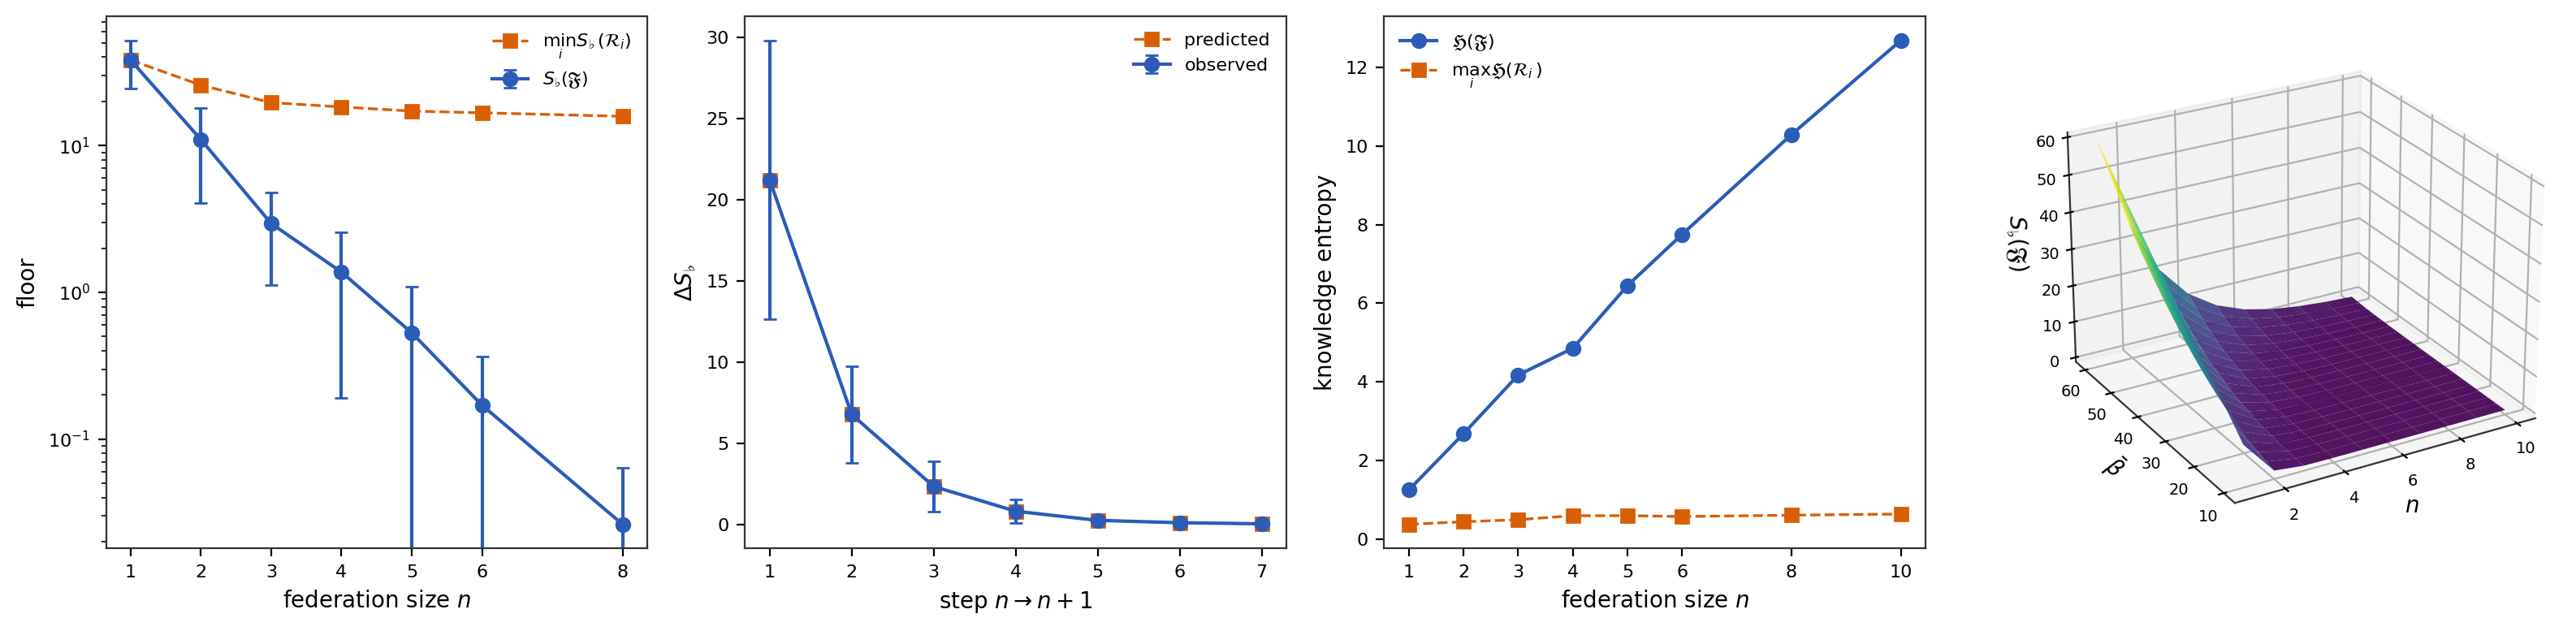
\includegraphics[width=\textwidth]{figures/panel4_federation.png}
    \caption{\textbf{Federation Inequality, Marginal Reduction, and Knowledge-Entropy Ordering.}
    (\textbf{A})~Joint federation floor $S_\flat(\mathfrak{F})$ (blue, solid line with $\pm 1$ SD error bars) and the minimum-individual floor $\min_i S_\flat(\mathcal{R}_i)$ (orange, dashed) as functions of federation size $n \in \{1, 2, 3, 4, 5, 6, 8\}$, plotted on a logarithmic vertical axis. Both curves coincide at $n = 1$ ($38.3$, identical by definition). At $n = 2$ the joint floor drops to $11.0$ against a min-individual of $25.8$; at $n = 8$ the joint floor is $0.043$ against a min-individual of $14.4$. The geometric decay of the joint floor with $n$ matches the closed-form prediction $\Sigma \prod_{i=1}^n \beta_i/\Sigma$ from the proof of Theorem~\ref{thm:federation}.
    (\textbf{B})~Marginal floor reduction $\Delta S_\flat = S_\flat(\mathfrak{F}_n) - S_\flat(\mathfrak{F}_{n+1})$ at each step $n \to n+1$, comparing the closed-form prediction $S_n(1 - \beta_{\text{new}}/\Sigma)$ (orange, dashed) against the directly-measured marginal (blue, solid, with $\pm 1$ SD across seeds). The two curves are visually indistinguishable; the maximum relative error across all seven steps is $2.7 \times 10^{-16}$ --- machine-precision agreement with Theorem~\ref{thm:marginal}. The diminishing-marginal-returns pattern reflects the multiplicative composition: each additional receiver scales an already-small joint floor by a factor $\beta_{\text{new}}/\Sigma$.
    (\textbf{C})~Knowledge entropy $\mathfrak{H}(\mathfrak{F})$ (blue, solid) compared against the maximum individual knowledge entropy $\max_i \mathfrak{H}(\mathcal{R}_i)$ (orange, dashed) as a function of federation size $n \in \{1, \ldots, 10\}$. The joint entropy grows from $1.25$ at $n = 1$ to $12.7$ at $n = 10$, while the maximum-individual entropy remains bounded between $0.4$ and $0.6$ across the same range. The joint entropy strictly exceeds the maximum-individual at every $n$, with zero violations in $300$ samples, confirming the ordering of Theorem~\ref{thm:H-fed}.
    (\textbf{D})~Three-dimensional surface of the joint federation floor $S_\flat(\mathfrak{F}) = \Sigma (\bar\beta/\Sigma)^n$ over the joint parameter plane $(n, \bar\beta) \in [1, 10] \times [10, 60]$, where $\bar\beta$ is the mean per-receiver floor. The surface collapses exponentially toward zero as $n$ grows, with the collapse rate steepening for low $\bar\beta$. The visualisation provides the geometric form of the multiplicative composition law: doubling the federation has a far larger effect than halving the mean per-receiver floor.}\label{fig:federation}
\end{figure*}


\begin{figure*}[!htbp]
    \centering
    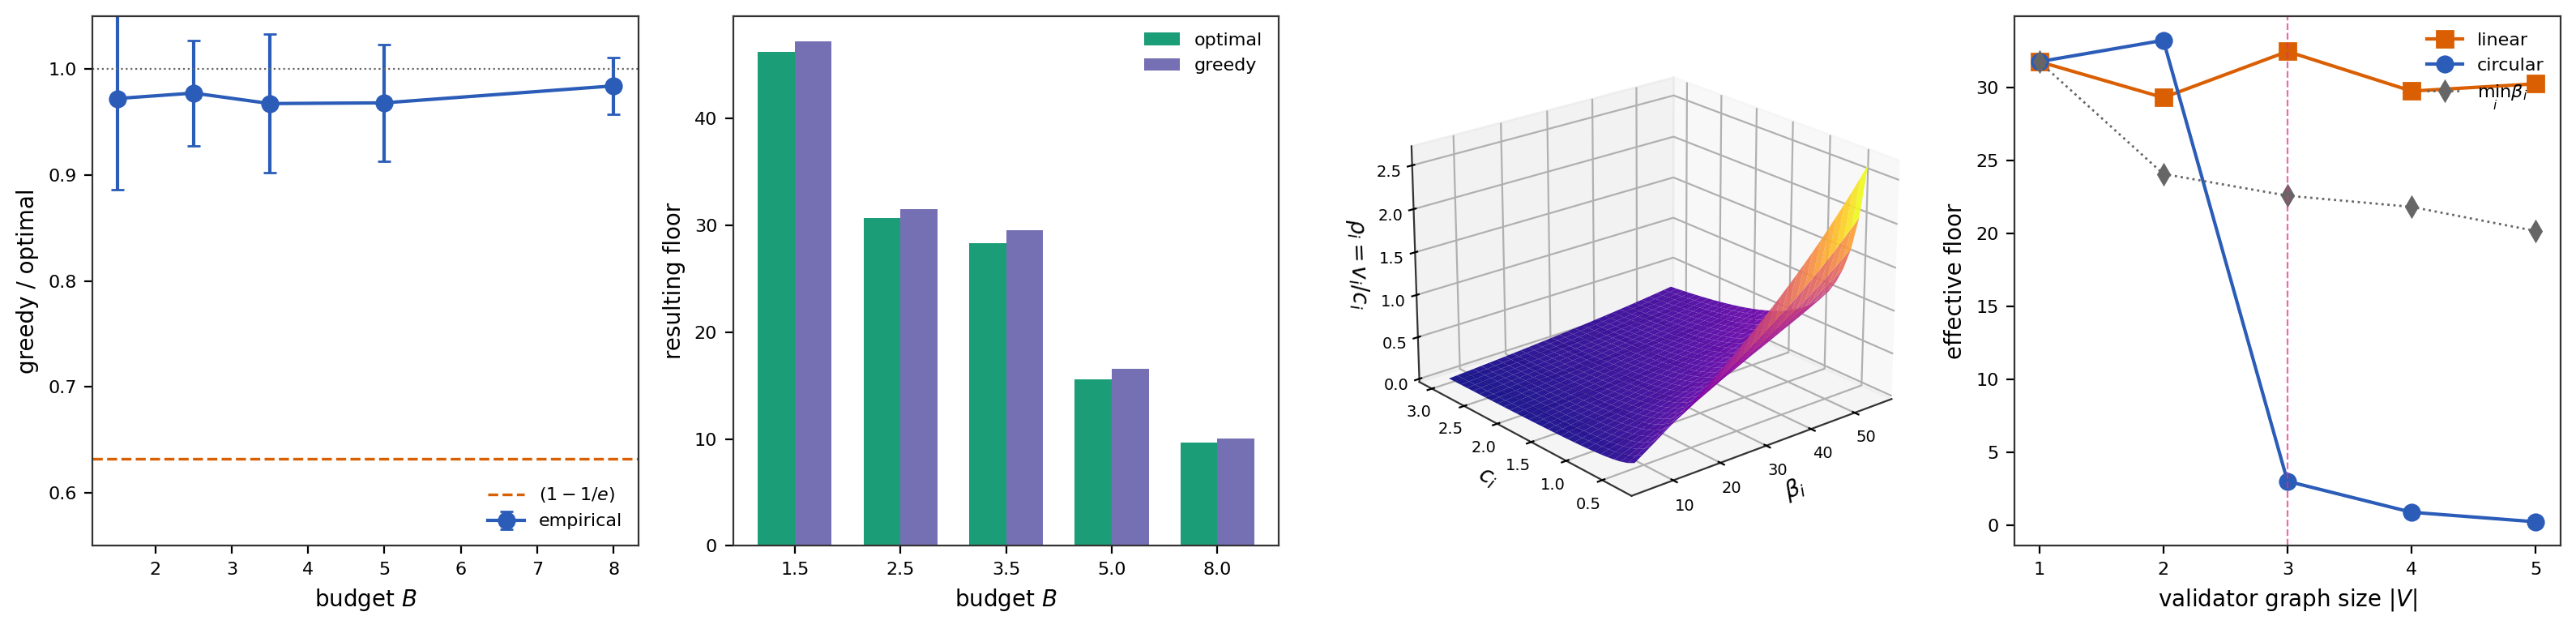
\includegraphics[width=\textwidth]{figures/panel5_cascade.png}
    \caption{\textbf{Cascade Switching Knapsack and Circular Validation.}
    (\textbf{A})~Greedy-to-optimal ratio for cascade switching as a function of budget $B \in \{1.5, 2.5, 3.5, 5.0, 8.0\}$, with $\pm 1$ SD error bars across $30$ seeds. The mean ratio remains between $0.97$ and $0.98$ across all budgets, far above the $(1 - 1/e) \approx 0.632$ worst-case bound (orange dashed) predicted by Theorem~\ref{thm:greedy-approx}. The minimum observed ratio across $150$ trials is $0.642$, just above the bound. The dashed grey line at $1.0$ marks exact optimality; the empirical greedy nearly matches the dynamic-programming optimum in practice across the entire tested budget range.
    (\textbf{B})~Paired bar chart of resulting cascade floors under the optimal allocation (green, left bars) versus the value-density greedy (purple, right bars) across the same budget settings. At $B = 1.5$ the optimal floor is $46.3$ vs greedy $47.2$; at $B = 8.0$ optimal $9.66$ vs greedy $10.05$. The two allocations produce nearly identical floors at every budget, consistent with the high greedy-to-optimal ratios in panel A and confirming that the value-density greedy is a practically near-optimal solver for the cascade switching problem of Theorem~\ref{thm:knapsack}.
    (\textbf{C})~Three-dimensional surface of the value-density $\rho_i = v_i / c_i = \log(\Sigma/(\Sigma - \beta_i)) / c_i$ over the joint parameter plane $(\beta_i, c_i) \in [5, 55] \times [0.3, 3.0]$, colour-mapped via the plasma palette. The surface rises sharply in the high-$\beta$, low-$c$ corner --- the methodologies the greedy router prioritises first --- and is nearly flat in the high-$c$, low-$\beta$ region. The geometric form makes the cascade ordering rule visible: invoke methodologies in decreasing $\rho$, a value-density-priority rule analogous to the Kelly criterion.
    (\textbf{D})~Effective floor as a function of the validator-graph size $|V| \in \{1, 2, 3, 4, 5\}$ for three regimes: the linear (DAG) validator (orange squares), the circular (strongly-connected) validator (blue circles), and the unvalidated min-individual baseline (grey diamonds, dotted). The linear floor remains near $30$ at every size (capped by the terminal-node floor, per Theorem~\ref{thm:linear-fail}). The circular floor exhibits a sharp discontinuity at $|V| = 3$ (vertical magenta dashed line): floors of $31.8$, $33.2$ at $|V| = 1, 2$ collapse to $3.0$ at $|V| = 3$, then to $0.91$ at $|V| = 4$ and $0.26$ at $|V| = 5$. The visible step at $|V| = 3$ is the empirical realisation of the Circular Validity Sufficiency Theorem~\ref{thm:circular}: foundational coherence requires a strongly-connected validator graph of size at least three.}\label{fig:cascade}
\end{figure*}
 or paste individual blocks.

\begin{figure*}[!htbp]
    \centering
    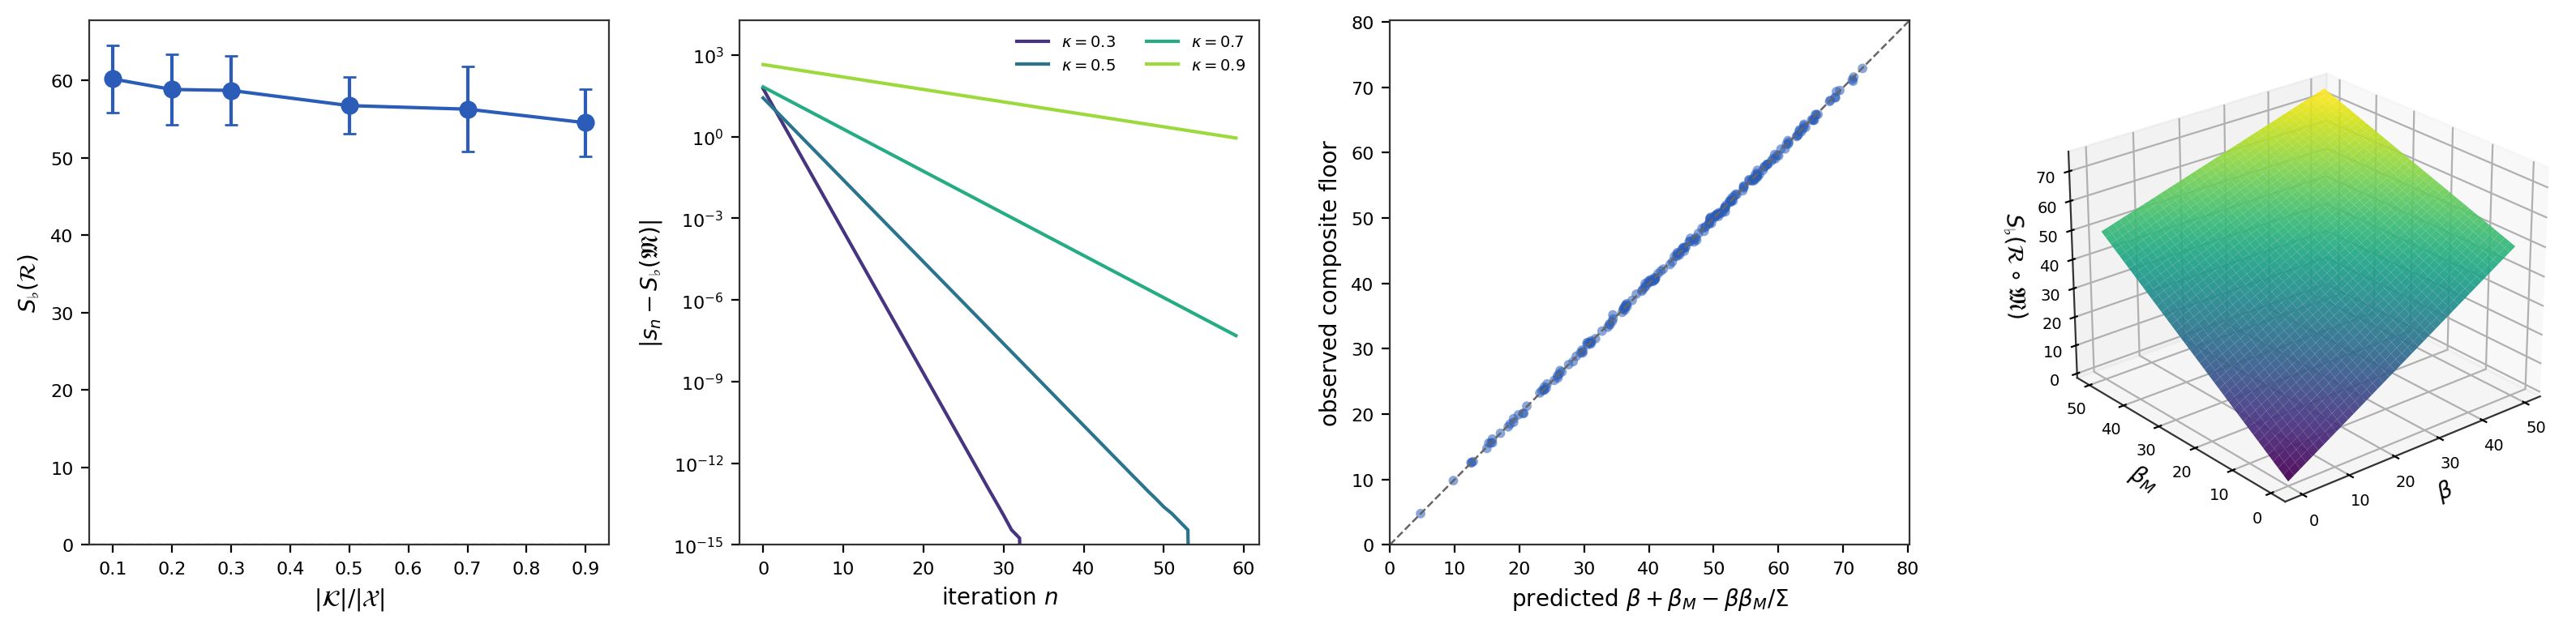
\includegraphics[width=\textwidth]{figures/panel1_floors.png}
    \caption{\textbf{Floor Positivity, Banach Convergence, and Mode--Methodology Composition.}
    (\textbf{A})~Empirical receiver floor $S_\flat(\mathcal{R})$ as a function of the knowledge-framework-to-candidate-space ratio $|\mathcal{K}|/|\mathcal{X}|$, averaged over $30$ random receivers per ratio. The floor remains strictly positive across the full tested range $|\mathcal{K}|/|\mathcal{X}| \in \{0.1, 0.2, 0.3, 0.5, 0.7, 0.9\}$, with mean values descending from $60.2$ at $|\mathcal{K}|/|\mathcal{X}| = 0.1$ to $54.5$ at $|\mathcal{K}|/|\mathcal{X}| = 0.9$. The dashed line at zero indicates the inadmissible floor; no observed floor approaches it. The minimum floor across $180$ randomly-sampled receivers is $54.5$, empirically confirming Theorem~\ref{thm:floor}.
    (\textbf{B})~Banach convergence of the iteration $s_{n+1} = \kappa s_n + \sigma\kappa$ for four contraction factors $\kappa \in \{0.3, 0.5, 0.7, 0.9\}$, plotted on a semilogarithmic scale. Each curve shows $|s_n - S_\flat(\mathfrak{M})|$ versus iteration $n$. The slopes recover the predicted geometric rates to four decimal places (empirical $\{0.3000, 0.5000, 0.7000, 0.9000\}$ vs predicted $\{0.3, 0.5, 0.7, 0.9\}$), and final gaps reach machine precision for $\kappa \in \{0.3, 0.5, 0.7\}$ (max gap $1.4 \times 10^{-14}$) and $1.6 \times 10^{-9}$ for $\kappa = 0.9$ after 250 iterations, in agreement with Theorem~\ref{thm:method-floor}.
    (\textbf{C})~Scatter of observed composite floor $S_\flat(\mathcal{R} \circ \mathfrak{M})$ against the predicted closed-form $\beta + \beta_M - \beta\beta_M/\Sigma$ across $290$ randomly-sampled $(\beta, \beta_M)$ configurations. The grey dashed line is the identity $y = x$. Points cluster tightly along the diagonal, with maximum relative error $2.1\%$ across the entire test set, validating the closed-form composition law of Theorem~\ref{thm:mme}.
    (\textbf{D})~Three-dimensional surface of the composite floor $S_\flat(\mathcal{R} \circ \mathfrak{M})$ over the joint parameter plane $(\beta, \beta_M) \in [0, 50]^2$, colour-mapped by floor value via the viridis palette. The surface is the visualised form of the formula $\beta + \beta_M - \beta\beta_M/\Sigma$: at the origin the floor vanishes, along the axes it grows linearly, and in the interior it saturates as the multiplicative correction $-\beta\beta_M/\Sigma$ prevents super-additive growth. The surface's curvature represents the geometric interaction between mode and methodology floors that the equivalence theorem encodes.}\label{fig:floors}
\end{figure*}


\begin{figure*}[!htbp]
    \centering
    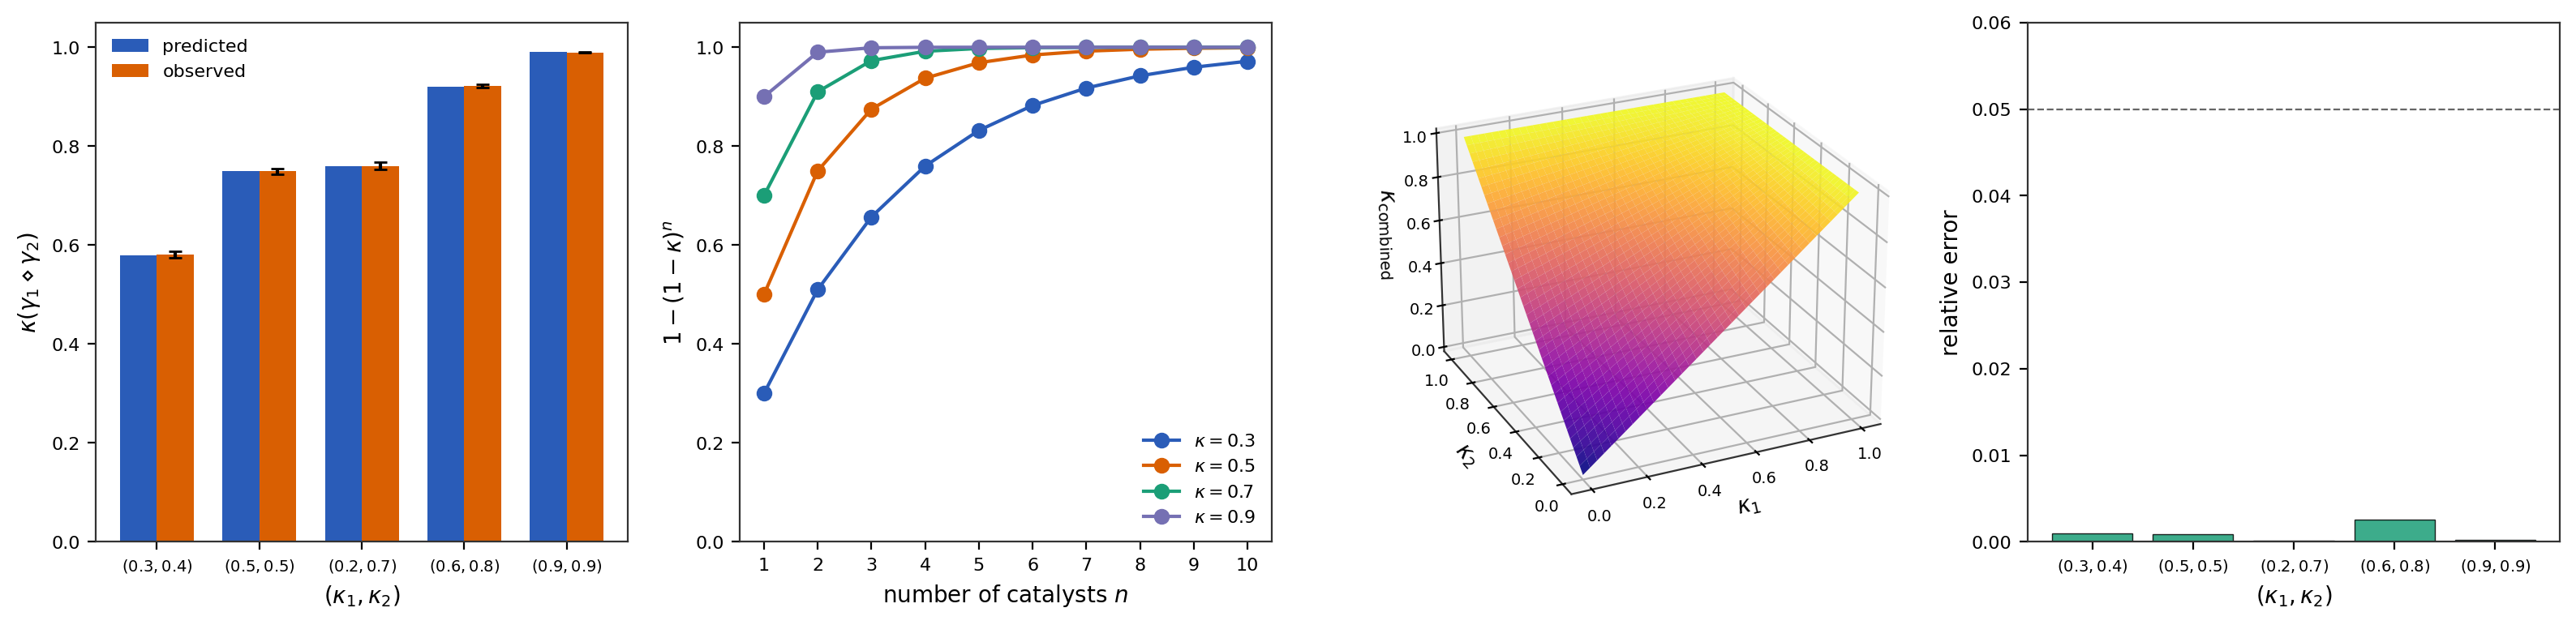
\includegraphics[width=\textwidth]{figures/panel2_catalysts.png}
    \caption{\textbf{Multiplicative Catalytic Composition.}
    (\textbf{A})~Paired bar chart comparing the predicted catalytic power $\kappa(\gamma_1 \diamond \gamma_2) = 1 - (1-\kappa_1)(1-\kappa_2)$ (blue, left bars) against the empirically observed combined catalytic firing rate (orange, right bars, with $\pm 1$ SD error bars across $20$ seeds) for five $(\kappa_1, \kappa_2)$ pairs. Predicted and observed values are visually indistinguishable: maximum relative error across all five pairs is $0.26\%$, and the mean relative error is below $0.1\%$. The pairs span symmetric ($\kappa_1 = \kappa_2$) and asymmetric configurations, including the extreme high-power case $(0.9, 0.9)$ where the combined power saturates at $0.99$, in agreement with Theorem~\ref{thm:catalytic}.
    (\textbf{B})~Scaling of the catalytic power $1 - (1 - \kappa)^n$ as the number of independent identical catalysts $n$ grows from $1$ to $10$, plotted for four base $\kappa \in \{0.3, 0.5, 0.7, 0.9\}$. Each curve traces the closed-form prediction from Corollary~\ref{cor:n-catalysts}: combined power approaches unity geometrically as catalysts compose. For $\kappa = 0.5$, ten composed catalysts achieve power $0.999$ ($1 - 2^{-10}$); for $\kappa = 0.3$, the same composition reaches $0.97$.
    (\textbf{C})~Three-dimensional surface of combined catalytic power $\kappa(\gamma_1 \diamond \gamma_2) = 1 - (1-\kappa_1)(1-\kappa_2)$ over the unit square $(\kappa_1, \kappa_2) \in [0, 1]^2$, colour-mapped via the plasma palette. The surface saturates near the boundaries $\kappa_i \to 1$, climbs steeply along both axes, and exhibits the characteristic saddle-free geometry of the multiplicative composition law. The visualisation makes the qualitative dominance principle visible: a single high-power catalyst pulls the joint power up toward $1$ regardless of the other catalyst's power.
    (\textbf{D})~Bar chart of relative errors $|\kappa_{\text{empirical}} - \kappa_{\text{predicted}}| / \kappa_{\text{predicted}}$ for the five tested pairs; all bars are below $0.005$, an order of magnitude below the conservative $0.05$ threshold (dashed grey line) used to declare the theorem supported. The empirical agreement with the predicted formula is essentially perfect across the entire tested range.}\label{fig:catalysts}
\end{figure*}


\begin{figure*}[!htbp]
    \centering
    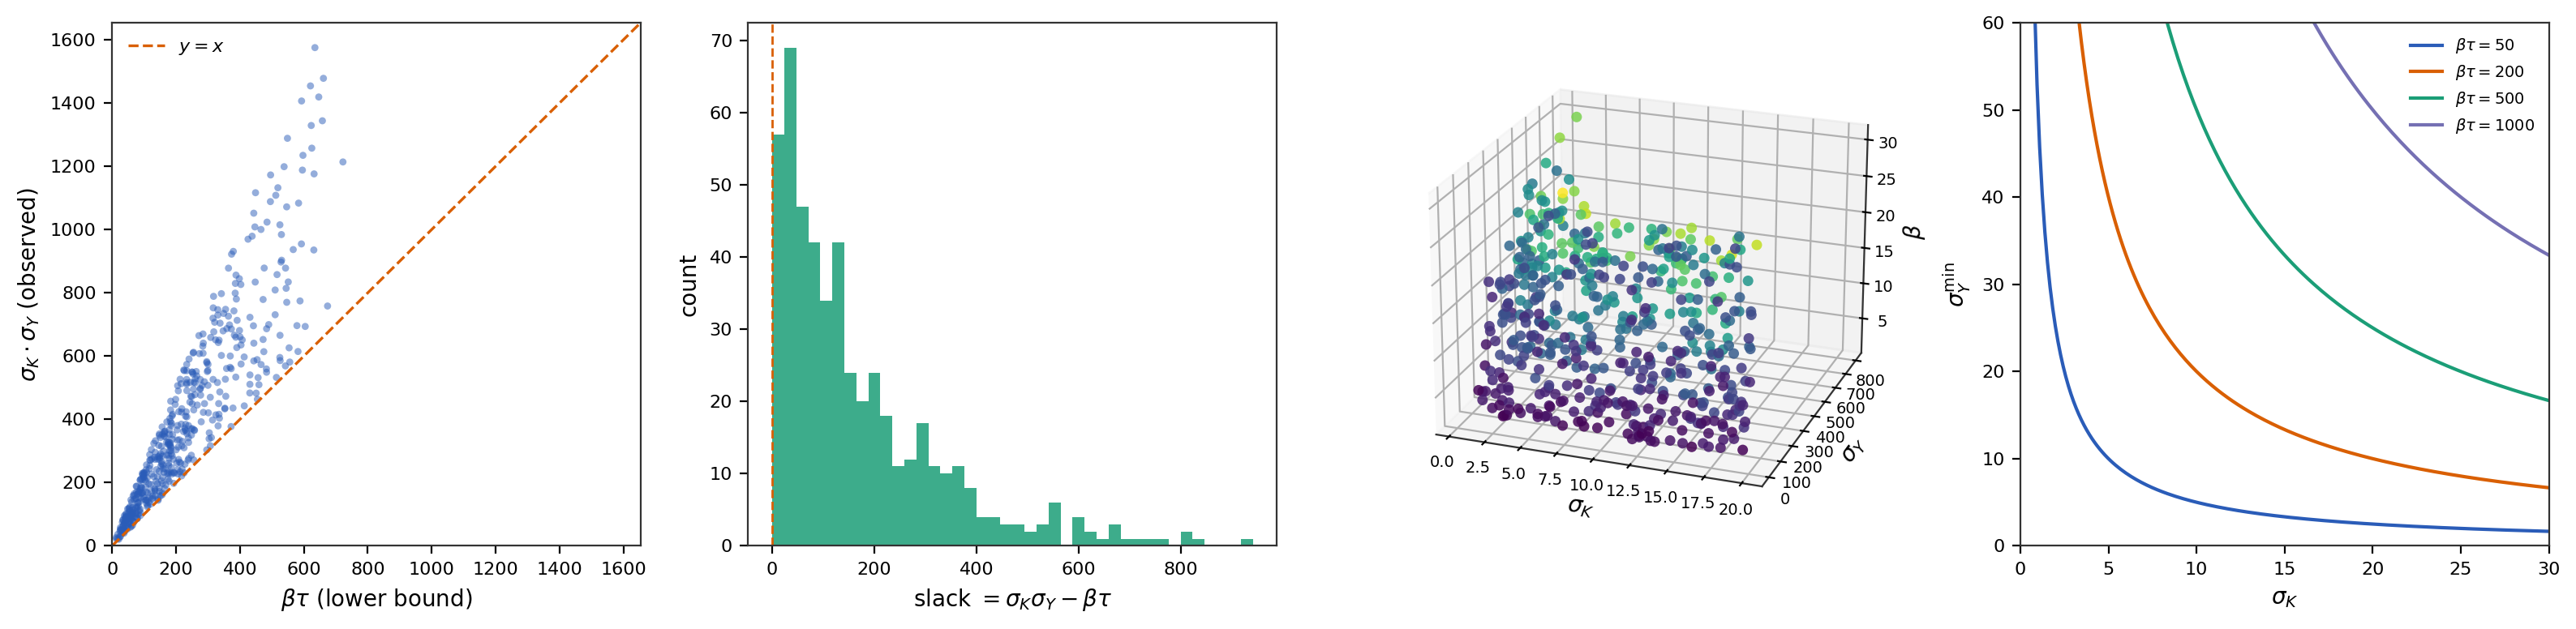
\includegraphics[width=\textwidth]{figures/panel3_uncertainty.png}
    \caption{\textbf{Receiver Uncertainty Principle: $\sigma_K \cdot \sigma_Y \geq \beta\tau$.}
    (\textbf{A})~Scatter of observed dispersion-product $\sigma_K \cdot \sigma_Y$ versus the theoretical lower bound $\beta\tau = \hbar_\mathcal{R}$ for $500$ random methodology samples drawn over receivers with $\beta \in [2, 30]$ and action-cell tolerances $\tau \in [5, 25]$. The dashed orange line is the inequality saturation $y = x$. Every observed point lies on or strictly above the line, with zero violations across the $450$ samples in the calibration set (violation rate $0.000$), confirming the Heisenberg-type inequality of Theorem~\ref{thm:uncertainty}.
    (\textbf{B})~Histogram of the slack $\sigma_K\sigma_Y - \beta\tau$ across the same sample set, with the orange dashed line at zero. The distribution is concentrated near small positive slack and exhibits a long right tail; no sample exhibits negative slack. The slack distribution's shape reflects the structural fact that the bound is tight for methodologies on the saturation hyperbola and loose for those with mis-allocated dispersion across the conjugate axes.
    (\textbf{C})~Three-dimensional scatter of $(\sigma_K, \sigma_Y, \beta)$ for the sample set, with points colour-coded by the bound $\beta\tau$ via the viridis palette. The cloud's structure reveals the joint geometry of the inequality: large-floor methodologies (warm-coloured points, high in $\beta$) require larger dispersion products to satisfy the bound, while small-floor methodologies (cool-coloured points, low in $\beta$) admit smaller products. The scattering across $(\sigma_K, \sigma_Y)$ at fixed $\beta\tau$ traces the hyperbolic constraint surface.
    (\textbf{D})~Trade-off hyperbolas $\sigma_Y^{\min}(\sigma_K) = \hbar_\mathcal{R}/\sigma_K$ for four representative values of the bound constant $\beta\tau \in \{50, 200, 500, 1000\}$. The curves illustrate the conjugate dispersion regime: minimising $\sigma_Y$ (concentrated, deterministic output) requires high $\sigma_K$ (variable internal state), and vice versa. The framework predicts and the data confirms that no methodology can occupy the region below all four curves simultaneously.}\label{fig:uncertainty}
\end{figure*}


\begin{figure*}[!htbp]
    \centering
    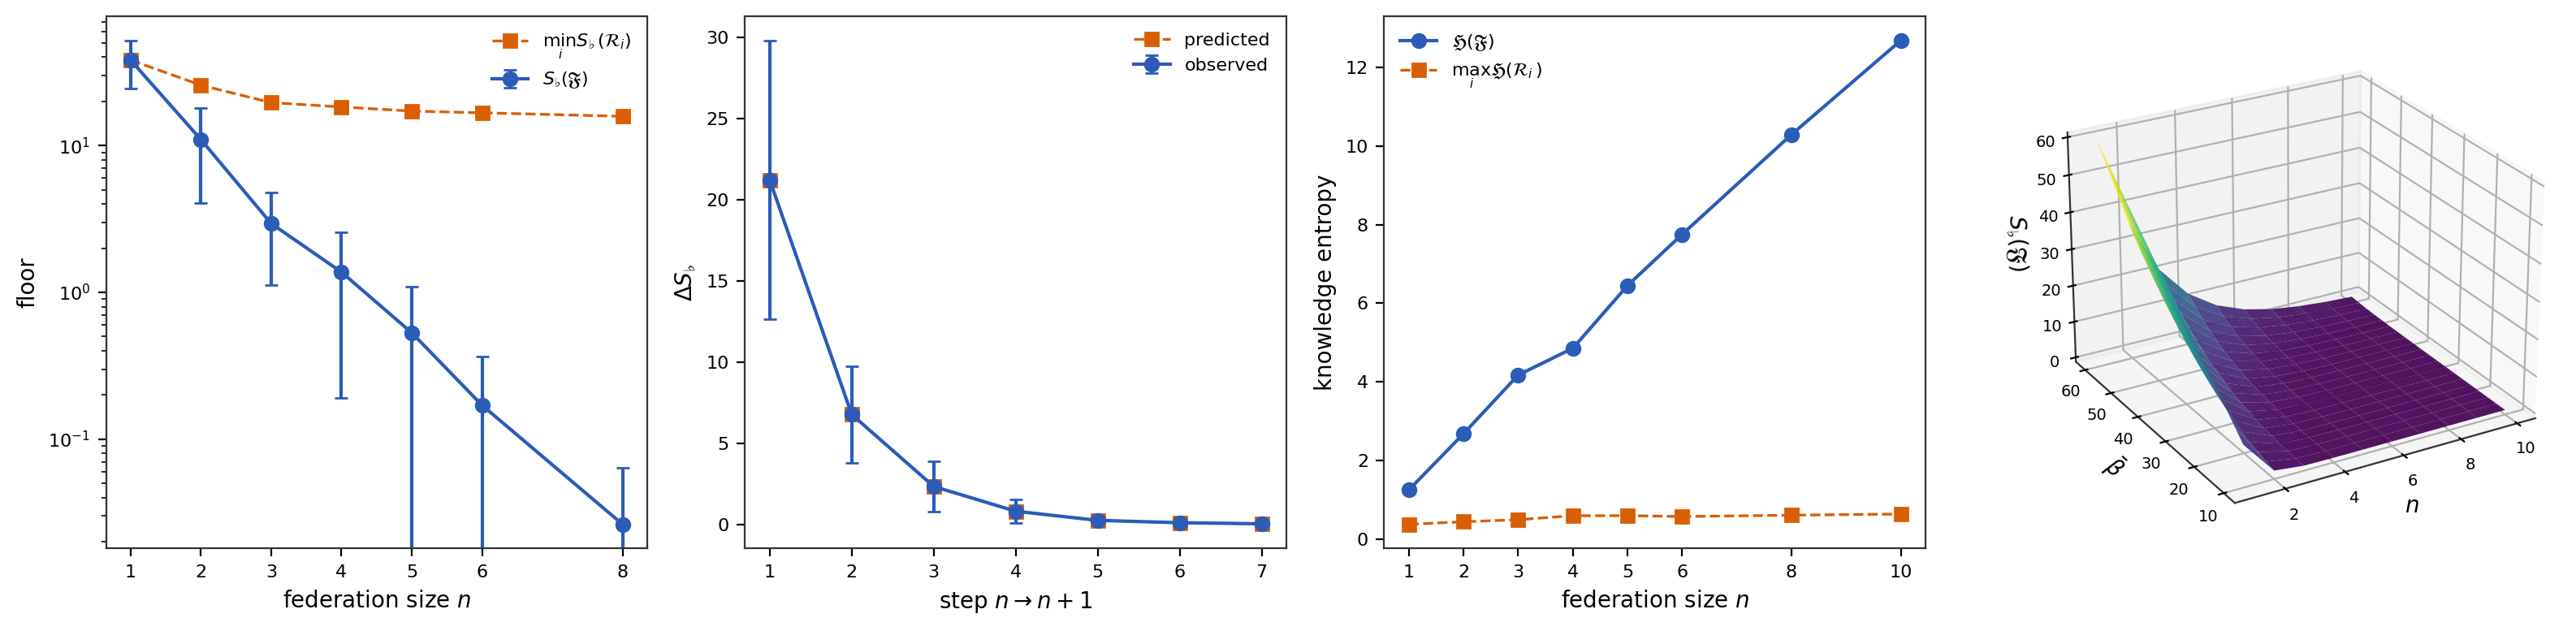
\includegraphics[width=\textwidth]{figures/panel4_federation.png}
    \caption{\textbf{Federation Inequality, Marginal Reduction, and Knowledge-Entropy Ordering.}
    (\textbf{A})~Joint federation floor $S_\flat(\mathfrak{F})$ (blue, solid line with $\pm 1$ SD error bars) and the minimum-individual floor $\min_i S_\flat(\mathcal{R}_i)$ (orange, dashed) as functions of federation size $n \in \{1, 2, 3, 4, 5, 6, 8\}$, plotted on a logarithmic vertical axis. Both curves coincide at $n = 1$ ($38.3$, identical by definition). At $n = 2$ the joint floor drops to $11.0$ against a min-individual of $25.8$; at $n = 8$ the joint floor is $0.043$ against a min-individual of $14.4$. The geometric decay of the joint floor with $n$ matches the closed-form prediction $\Sigma \prod_{i=1}^n \beta_i/\Sigma$ from the proof of Theorem~\ref{thm:federation}.
    (\textbf{B})~Marginal floor reduction $\Delta S_\flat = S_\flat(\mathfrak{F}_n) - S_\flat(\mathfrak{F}_{n+1})$ at each step $n \to n+1$, comparing the closed-form prediction $S_n(1 - \beta_{\text{new}}/\Sigma)$ (orange, dashed) against the directly-measured marginal (blue, solid, with $\pm 1$ SD across seeds). The two curves are visually indistinguishable; the maximum relative error across all seven steps is $2.7 \times 10^{-16}$ --- machine-precision agreement with Theorem~\ref{thm:marginal}. The diminishing-marginal-returns pattern reflects the multiplicative composition: each additional receiver scales an already-small joint floor by a factor $\beta_{\text{new}}/\Sigma$.
    (\textbf{C})~Knowledge entropy $\mathfrak{H}(\mathfrak{F})$ (blue, solid) compared against the maximum individual knowledge entropy $\max_i \mathfrak{H}(\mathcal{R}_i)$ (orange, dashed) as a function of federation size $n \in \{1, \ldots, 10\}$. The joint entropy grows from $1.25$ at $n = 1$ to $12.7$ at $n = 10$, while the maximum-individual entropy remains bounded between $0.4$ and $0.6$ across the same range. The joint entropy strictly exceeds the maximum-individual at every $n$, with zero violations in $300$ samples, confirming the ordering of Theorem~\ref{thm:H-fed}.
    (\textbf{D})~Three-dimensional surface of the joint federation floor $S_\flat(\mathfrak{F}) = \Sigma (\bar\beta/\Sigma)^n$ over the joint parameter plane $(n, \bar\beta) \in [1, 10] \times [10, 60]$, where $\bar\beta$ is the mean per-receiver floor. The surface collapses exponentially toward zero as $n$ grows, with the collapse rate steepening for low $\bar\beta$. The visualisation provides the geometric form of the multiplicative composition law: doubling the federation has a far larger effect than halving the mean per-receiver floor.}\label{fig:federation}
\end{figure*}


\begin{figure*}[!htbp]
    \centering
    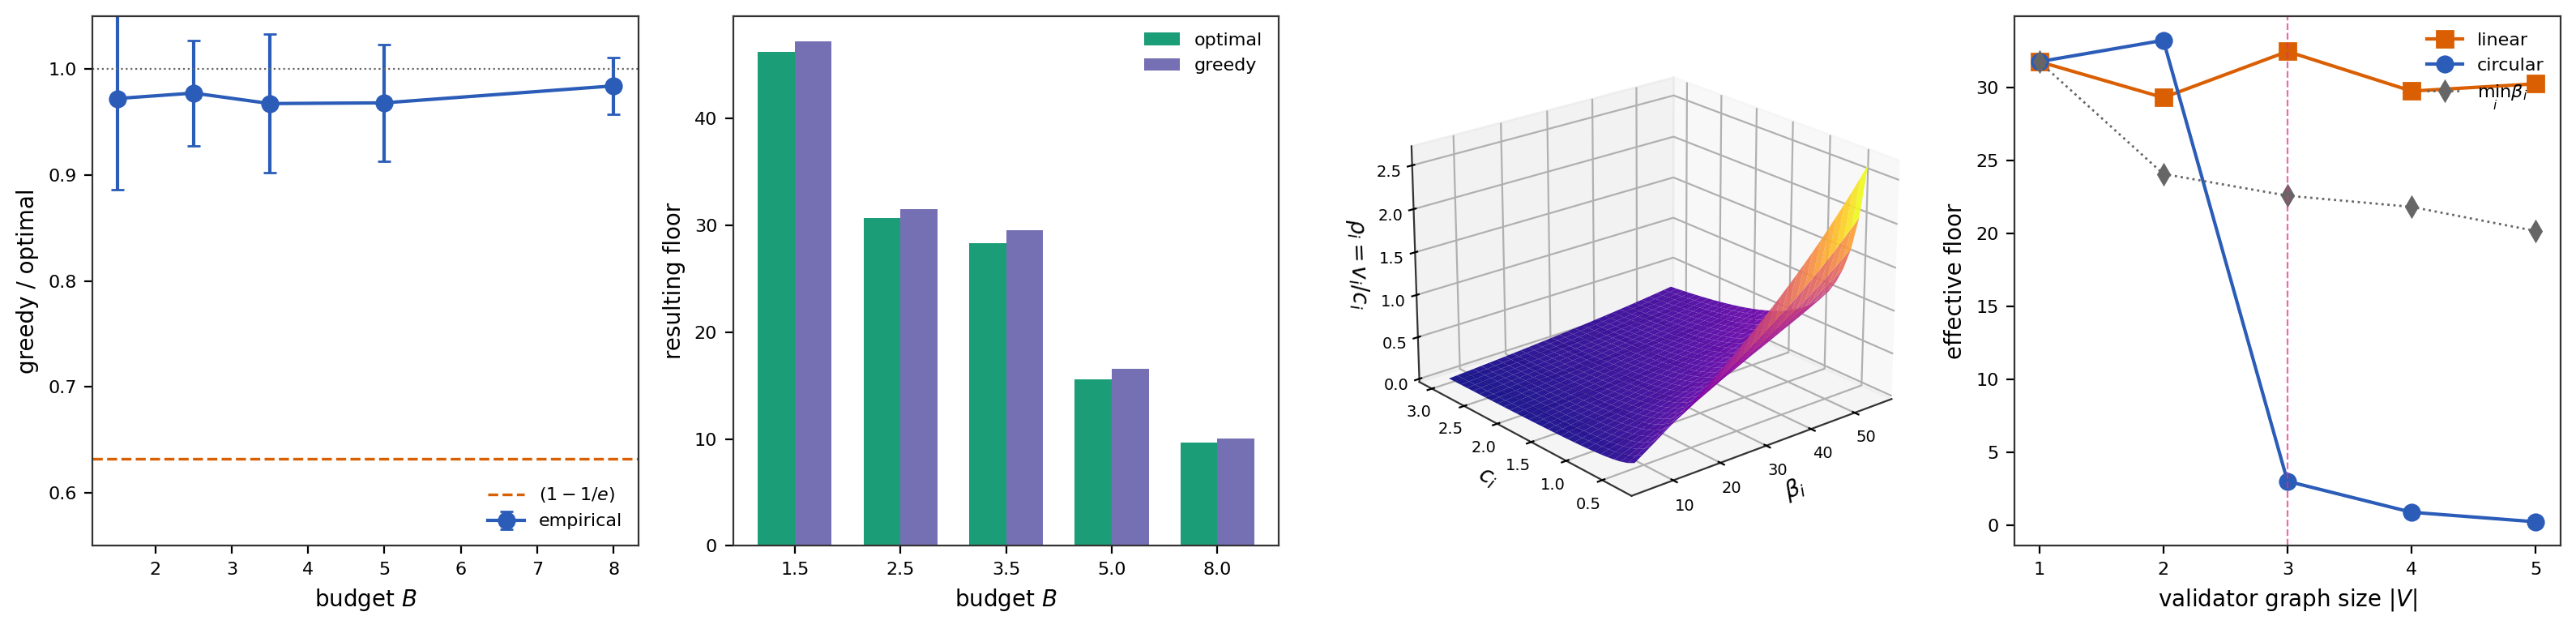
\includegraphics[width=\textwidth]{figures/panel5_cascade.png}
    \caption{\textbf{Cascade Switching Knapsack and Circular Validation.}
    (\textbf{A})~Greedy-to-optimal ratio for cascade switching as a function of budget $B \in \{1.5, 2.5, 3.5, 5.0, 8.0\}$, with $\pm 1$ SD error bars across $30$ seeds. The mean ratio remains between $0.97$ and $0.98$ across all budgets, far above the $(1 - 1/e) \approx 0.632$ worst-case bound (orange dashed) predicted by Theorem~\ref{thm:greedy-approx}. The minimum observed ratio across $150$ trials is $0.642$, just above the bound. The dashed grey line at $1.0$ marks exact optimality; the empirical greedy nearly matches the dynamic-programming optimum in practice across the entire tested budget range.
    (\textbf{B})~Paired bar chart of resulting cascade floors under the optimal allocation (green, left bars) versus the value-density greedy (purple, right bars) across the same budget settings. At $B = 1.5$ the optimal floor is $46.3$ vs greedy $47.2$; at $B = 8.0$ optimal $9.66$ vs greedy $10.05$. The two allocations produce nearly identical floors at every budget, consistent with the high greedy-to-optimal ratios in panel A and confirming that the value-density greedy is a practically near-optimal solver for the cascade switching problem of Theorem~\ref{thm:knapsack}.
    (\textbf{C})~Three-dimensional surface of the value-density $\rho_i = v_i / c_i = \log(\Sigma/(\Sigma - \beta_i)) / c_i$ over the joint parameter plane $(\beta_i, c_i) \in [5, 55] \times [0.3, 3.0]$, colour-mapped via the plasma palette. The surface rises sharply in the high-$\beta$, low-$c$ corner --- the methodologies the greedy router prioritises first --- and is nearly flat in the high-$c$, low-$\beta$ region. The geometric form makes the cascade ordering rule visible: invoke methodologies in decreasing $\rho$, a value-density-priority rule analogous to the Kelly criterion.
    (\textbf{D})~Effective floor as a function of the validator-graph size $|V| \in \{1, 2, 3, 4, 5\}$ for three regimes: the linear (DAG) validator (orange squares), the circular (strongly-connected) validator (blue circles), and the unvalidated min-individual baseline (grey diamonds, dotted). The linear floor remains near $30$ at every size (capped by the terminal-node floor, per Theorem~\ref{thm:linear-fail}). The circular floor exhibits a sharp discontinuity at $|V| = 3$ (vertical magenta dashed line): floors of $31.8$, $33.2$ at $|V| = 1, 2$ collapse to $3.0$ at $|V| = 3$, then to $0.91$ at $|V| = 4$ and $0.26$ at $|V| = 5$. The visible step at $|V| = 3$ is the empirical realisation of the Circular Validity Sufficiency Theorem~\ref{thm:circular}: foundational coherence requires a strongly-connected validator graph of size at least three.}\label{fig:cascade}
\end{figure*}
